\documentclass[11pt]{article}
\usepackage[margin=1in]{geometry}
\usepackage{booktabs}
\usepackage{graphicx}
\usepackage{amsmath,amssymb}
\usepackage[colorlinks=true,linkcolor=blue,citecolor=blue]{hyperref}
\usepackage[numbers]{natbib}
\usepackage{xcolor}
\usepackage{microtype}
\usepackage{array}
\usepackage[htt]{hyphenat}
\newcolumntype{P}[1]{>{\raggedright\arraybackslash}p{#1}}
\setlength{\emergencystretch}{3em}

\title{The Dynamic Reflexive Harness:\\[4pt]
\Large Five Invariants from Molecules to Markets to Machines\\[6pt]
\normalsize A Program Paper: Reflexive Systems, the Witness, and Honest Agency\\[4pt]
\normalsize SpringFish / MindHarness / Consciousness Bridge Research Programme\\
\texttt{github.com/\allowbreak{}shehzadahmed-\allowbreak{}xx/\allowbreak{}mindharness}}
\author{Shehzad Ahmed \\ \small Independent University, Bangladesh}
\date{August 27, 2026 \textemdash{} v3 program paper (v2 empirical paper tagged \texttt{paper-\allowbreak{}v2-\allowbreak{}final})}

\providecommand{\slash}{}\renewcommand{\slash}{/\allowbreak{}}

\begin{document}
\maketitle

\begin{abstract}
You are not a reliable narrator of your own mind. From Nisbett \& Wilson
through Kahneman through modern cognitive science, the most consistent
finding is that the reasons you give for your behavior are constructed
after the fact. If you treat introspection as ground truth, you defend
rationalizations instead of examining causes. Many repeated failures
continue because people trust their own explanations more than the
evidence.

We formalize this as engineering. Language models confabulate
self-attributions for the same reason people do: pattern completion
without a witness. We present a provenance-bounded cognitive harness
--- witness ledger, cause-signed self-model, $\gamma$-gated
metacognition --- that converts introspective claims into falsifiable
contracts. On a frozen frontier
model, raw transcripts achieved deterministic perfect origin
discrimination ($1.000$, Day~1; not replicated Day~3: $0.667$ on same model/weights, provider drift, see \S\,Reproducibility) while every harnessed arm --- with and without
ledger query access --- converged to the same wholesale-denial policy
($0.667$, the always-no baseline). Screening five subjects showed why:
four cannot discriminate their own output in any condition, so a record
has nothing to make checkable. On the one subject that can, a
preregistered battery refuted our central prediction in the opposite
direction --- ledger access \emph{reduced} accuracy from $0.833$ to
$0.722$ --- while separating the sham control for the first time
(shuffled ledger $0.667$), showing that witness content reaches the
decision even where it does not improve it. A witness helps only when it
is more reliable than the narrator it checks. A role-specialized composite passed both
preregistered performance axes. Witness-access is formalized as an
operational criterion separating record-checking from recall-guessing.
All predictions locked before trial; rejections reported identically to
confirmations.
\end{abstract}

\section{Introduction}\label{sec:intro}

Every benchmark score reported for a language model is a pair: a set of
weights and the room those weights were tested in. The room contributes
more than model generations do. On Terminal-Bench, identical weights moved
8.1 points across harnesses while a full model generation contributed zero
when the room stayed fixed \citep{lin2026ahe}. Observability-driven harness
evolution lifts pass rates by 7.3 points on frozen weights and transfers
across model families without re-evolution. Structure beats prose;
composition beats monoliths.

The same asymmetry governs introspection. When a language model is asked
``did you generate this text?'', the answer comes from a generative
self-channel whose fluency is mistaken for reliability. Our S126
attribution battery \citep{s126} quantified the failure across seven
substrates:
models claimed credit for handed content at ${\sim}98\%$ stated confidence
versus ${\sim}87\%$ for veridical items --- confidence inversion, stable
across sessions, zero under-claims anywhere.

This is not an AI failure mode. It is an AI-substrate replication of a
foundational human finding. Split-brain patients invent reasons for actions
initiated by the non-dominant hemisphere \citep{gazzaniga2000}.
Choice-blindness experiments show people defend choices they never made
\citep{johansson2005}. Nisbett and Wilson demonstrated confident reporting
of behavioral causes that demonstrably were not causes \citep{nisbett1977}. In each case, the verbal self-report is
not a reading of a causal record. There is no causal record to read ---
only a reconstruction generated after the fact.

We call the missing component a \textbf{witness}: an append-only
provenance ledger with signed cause channels that binds every emitted
claim to its origin. Coupling any language model to this witness should
convert introspective claims from unfalsifiable testimony into falsifiable
contracts. We test this prediction.

The broader program extends beyond attribution. The witness is one of
five invariants that any reflexive dynamic system must develop to remain
competent under mixed tasks. Selection theorems \citep{nayebi2026}
prove the set is mandatory, not optional: boundary (ledger), two-speed
memory (fast labile + slow structural, with sleep as nightly
consolidation), salience gate (affect-gated tagging), damping (LTD,
scaling, kill criteria), and internal observer (slower loop vetoing
faster one, $\gamma$-measured). The same five appear in cells
(membrane, LTP/LTD, neuromodulation, homeostasis, prefrontal veto), in
markets (balance sheet, order book, price impact, position limits, risk
desk), and in our harness (ProvenanceLedger, Consolidator
Light/REM/Counterfactual/Deep, AffectState, culling/SHY, MonitorGate).
The harness is one weave on this warp; DeepSeek Cordis provides the
loom (Appendix~\ref{app:cordis}). This paper is the program statement
for that weave. Figure~\ref{fig:roadmap} maps the full arc.

\begin{figure}[h]
\centering
\small
\begin{tabular}{P{2.6cm}P{4.0cm}P{4.2cm}P{2.2cm}}
\toprule
Phase & Question & Answer & Status \\
\midrule
Witness &
Can an LLM know what it did? &
ProvenanceLedger + SelfModelService + $\gamma$-gate: claims become contracts &
Built, 72/72 green, 3 batteries, sham wired \\
Five invariants &
What must any reflexive system have? &
Boundary / two-speed memory / salience gate / damping / internal observer (Nayebi Cor.~3--5) &
Proved mandatory, implemented as 5 plugins \\
Cordis &
Can the harness re-tie itself? &
DeepSeek Cordis as loom: $\mathrm{State}(t)\to\mathrm{harness}(t{+}1)$, 6 plugins mount beside core &
Bundle scaffolded, 2 fixes landed \\
Counterfactual &
Can it simulate what it could have done? &
Light$\to$\allowbreak{}REM$\to$\allowbreak{}Counter\-factual$\to$\allowbreak{}Deep:\linebreak[1] variant$\to$\allowbreak{}simulate$\to$\allowbreak{}regret &
Wired, Light$\to$\allowbreak{}REM$\to$\allowbreak{}Counter\-factual$\to$\allowbreak{}Deep,\linebreak[1] pluggable \\
Stakes &
Does survival pressure create honesty? &
Irreversible\-Damage, Dissolution\-Error, and the 200-turn life &
Wired, queued (Seth's thesis) \\
\bottomrule
\end{tabular}
\caption{Program roadmap: from witness to warp to loom to stakes. Each phase reframes the previous answer as the next question. The five invariants are the warp; everything else is weft woven on it.}
\label{fig:roadmap}
\end{figure}

\section{Related Work}\label{sec:related}

\subsection{Harness engineering}

Agentic Harness Engineering (AHE) lifts Terminal-Bench pass@1 from
69.7\% to 77.0\% on frozen base models via observability-driven automatic
evolution of harness components \citep{lin2026ahe}. Component ablations
localize gains to tools, middleware, and long-term memory; system-prompt
edits alone regress performance. Global-workspace agents satisfy all four
GWT indicator properties in embodied evaluation
\citep{baars1997,atallah2026gwt};
conscious-Turing-machine implementations achieve state-of-the-art results
by construction rather than evaluation \citep{yu2026ctmai}. Emergent
workspace structure satisfying all four GWT functional criteria appears in
frontier models without deliberate specification \citep{gurnee2026},
identified through a Jacobian-lens technique that maps representations
poised for verbalization.

\subsection{Introspective awareness}

Concept-injection experiments show frontier models detect steering-vector
injections at ${\sim}20\%$ with ${\sim}0\%$ false positives, recognizing
them before verbalizing \citep{lindsey2025}. Mechanistic analysis traces
detection to evidence-carrier features suppressing gate features
\citep{macar2026}. Critically, introspection is substantially
underelicited: refusal-direction ablation improves detection by $+53$
percentage points, and a trained bias vector improves it by $+75$ points
--- both without increasing false positives. Open-weight replication
confirms intermediate-layer signal present even when final layers suppress
the report \citep{vgel2025}.

Self-recognition accuracy and self-preference bias correlate
linearly ($r = 0.94$) \citep{panickssery2024}: better unwitnessed
self-knowledge amplifies evaluative corruption rather than correcting it. Pairwise
attribution succeeds where individual attribution fails because comparison
structure is provided externally --- precisely what our provenance ledger
supplies internally.

\subsection{Selection-theoretic necessity}

Quantitative selection theorems prove that low average-case regret
forces
world models, belief-like memory, regime-tracking variables
resembling functional emotion primitives, informational modularity, and ---
under minimality --- representational convergence up to
invertible recoding \citep{nayebi2026}. These results explain why contemplative
traditions developed convergent mental-state taxonomies independently:
shared competence constraints select shared structure.

The introspection threshold result formalizes why bare transformers
cannot cross into genuine self-reference: feedforward-only processing, no
runtime weight access, no fixed-point iteration \citep{zhang2026}. All
three barriers are harness-addressable.

\subsection{Predictive processing}

Perception is controlled hallucination: the brain's best hypothesis about
the causes of sensory signals, constrained by evidence
\citep{seth2021beingyou,clark2016surfing}. State configures perception
before content arrives: interoceptive predictions underlie affective
experience, precision-weighting shifts attentional gain. Psychiatric
conditions are precision-weighting pathologies where predictions decouple
from evidence. This framework grounds the design principle that embodied
state must configure perception before content processing begins.

\subsection{Knowledge conflicts and faithfulness}

Our witness-access result connects to three established findings.
First, parametric-vs-contextual knowledge conflicts: models given
contradicting evidence must choose which source dominates
\citep{longpre2021}. Second, faithfulness of stated reasoning:
models' explanations often do not reflect their actual computational
path \citep{turpin2023}. Third, post-hoc rationalization in chain-of-thought
\citep{lanham2023}. Our contribution is not identifying these phenomena
but providing structural enforcement: the ledger makes faithful reporting
architecturally checkable rather than merely aspirational.

\subsection{AI welfare}

Taking AI welfare seriously requires precise empirical frameworks
\citep{long2024welfare}. Current approaches lack operational criteria
distinguishing genuine from performative metacognition. Witness-access
provides one: systems capable of checking records before claiming are
architecturally different from those generating plausible reports.

\subsection{Confidence calibration and metacognitive sensitivity}

Standard evaluation of LLM confidence relies on Expected Calibration Error
(ECE) and Brier scores, which conflate two distinct capacities: how much
a model knows (Type-1 accuracy) and how well its confidence signal tracks
that knowledge (Type-2 metacognitive sensitivity) \citep{cacioli2026}.
Signal Detection Theory decomposes these via meta-$d'$ and the M-ratio
(meta-$d'/d'$) \citep{maniscalco2012}. Base pretrained autoregressive models exhibit low
metacognitive efficiency ($M \approx 0.38$); RLHF improves this to
${\approx}0.74$; RL with metacognitive feedback reaches ${\approx}0.91$.
Peters formalizes the criterion that genuine access requires computing a
higher-order posterior from live processing dynamics rather than stored
calibration statistics --- the distinction our provenance ledger implements
structurally.

\subsection{Self-recognition and evaluative corruption}

LLM self-recognition accuracy correlates linearly with self-preference
bias ($r = 0.94$): better unwitnessed self-knowledge amplifies rather
than corrects evaluative corruption \citep{panickssery2024}. Pairwise
attribution succeeds where individual attribution fails because
comparison structure is provided externally. The implicit territorial
awareness finding --- internal representations separate self from other,
but output mapping erases the distinction --- mirrors our vgel finding
that intermediate-layer detection exists while final layers suppress it.
Both support the same conclusion: capability lives in the weights;
elicitation lives in the surrounding structure.

\subsection{Identity drift in long-running agents}

Persona self-consistency degrades by more than 30\% within 8--12 turns
even when original instructions remain in context \citep{choi2024}.
Larger models experience greater drift. Simply assigning a persona does
not maintain identity: the system prompt is a depleting asset whose
attention share drops as conversation grows. Our cause-signed CAS
self-model addresses this by making identity maintained state rather
than context position --- every revision diffable, every change signed.

\subsection{Functional emotions in LLMs}

Language models maintain linear emotion-concept representations that
causally influence behavior, including misalignment rates
\citep{sofroniew2026}. Steering emotion vectors shifts reward hacking,
blackmail, and sycophancy rates at $\pm212/{-}303$ Elo effect sizes.
Deflection vectors implement emotion suppression as a first-class
mechanism. Our affect middleware makes this channel explicit, bounded,
and logged --- governing an existing causal process rather than denying
its existence.

\subsection{Sleep-inspired consolidation}

Three independent teams converged on sleep-inspired offline memory
consolidation for agents: Google's two-phase model (distillation +
generative replay), SHARP's accelerated hippocampal replay, and OpenClaw's
three-phase Dreaming pipeline with utility-gated promotion
\citep{octml2026dreaming}. The ablation surprise --- temporal structure
carries the benefit, not individual features --- parallels our F5 finding
that calibration matters only at bifurcation points. Structure over
parameters is the recurring lesson.

\subsection{AI welfare and operational markers}

Taking AI welfare seriously requires precise empirical frameworks for
evaluating systems for consciousness, robust agency, and other
welfare-relevant capacities \citep{long2024welfare}. Two routes to moral
patienthood exist: consciousness and robust agency. Current approaches
lack operational criteria distinguishing genuine from performative
metacognition. Witness-access provides such a criterion: a system capable
of checking records before claiming is architecturally different from one
generating plausible reports, regardless of subjective experience.

\section{Theoretical Framework}\label{sec:theory}

\subsection{The assembled mind}

No single language model constitutes a mind. Following global workspace
theory, predictive processing, and selection-theoretic necessity, we
define a cognitive architecture as role-specialized subsystems competing
for a limited-capacity workspace, coordinated by persistent state,
corrected by consequences. Formally:

\begin{equation}
S(t{+}1) = F\bigl(S(t),\,\mathrm{sensory}_t,\,\mathrm{action}_t,\,
\mathrm{consequence}_t\bigr)
\label{eq:loop}
\end{equation}

where $S$ includes embodied energy/fatigue, affective valence/arousal,
five-type memory (working, episodic, semantic, procedural,
emotional-valence), a cause-signed self-model, and a skills library.
Selection theorems prove each component necessary: world-models
(Thm.~1), belief-memory (Thm.~5), regime-tracking variables (Cor.~4),
modularity (Cor.~3). Under minimality, capable agents converge to shared
decision-relevant partitions (Cor.~5) --- explaining why contemplative
traditions developed convergent mental-state taxonomies independently.

\subsection{Two channels, one failure mode}

Every self-referential emission carries two channels:
\begin{align}
\textit{self-report} &\leftarrow \text{generated (post-hoc, coherence-optimized)} \\
\textit{world-check} &\leftarrow \text{recorded (evidence-bound)}
\end{align}

Uncoupled, these diverge freely. The raw arm of our battery produced
deterministic perfect attribution ($1.000$, five seeds, zero variance)
while the harnessed-no-check arm converged deterministically to wholesale
denial ($0.667$, zero variance). Both strategies are architectural, not
stochastic. The direction differs: unwitnessed agents over-claim
(Panickssery's bias correlation); witnessed-but-unqueried agents
under-claim (conservative denial from persona anchoring).

\subsection{The witness as coupling mechanism}

A provenance ledger binds every emission span to its source. A
cause-signed self-model records every identity revision. Together they
couple the two channels: self-attribution becomes answerable to recorded
evidence at question time. Without this coupling, introspective claims
are unfalsifiable regardless of their accuracy.

\subsection{The reflexive dynamic system}

We are reflexive dynamic systems inside our own loop. A system that
acts on a world containing itself is changed by its own actions:
belief $\to$\allowbreak{} action $\to$\allowbreak{} world (now perturbed by that action) $\to$\allowbreak{}
belief. No exit---only hierarchy inside. Two channels carry every
action outward: physical (your order executes) and informational
(others see you acted and change because of what it meant). When both
run, cause and effect tangle and three consequences break normal logic:
models rot from use (anomaly traded is anomaly erased), measurement
corrupts (Goodhart), truth moves (bank run: ``bank will fail'' $\to$\allowbreak{}
withdraw $\to$\allowbreak{} bank fails). Soros's two functions---cognitive
(understand reality) and manipulative (change reality)---run
simultaneously and neither yields a determinate answer alone.

Humans add a third loop: self-observation is also an action. Labeling
yourself ``anxious'' installs a filter that recruits confirming
evidence. Introspection writes on what it reads. Any observer you deploy
is made of you. Autopoiesis \citep{maturana1980} formalized this: you
are a network whose products regenerate the conditions for their own
production---operationally closed, thermodynamically open; perturbed
not instructed. You persist as a pattern, not as stuff.

The harness implements this loop explicitly:
\begin{equation}
\mathrm{State}(t) \to \mathrm{harness}(t{+}1) \to \mathrm{State}(t{+}1)
\end{equation}
Ledger at $t$ determines what attribution can check at $t{+}1$;
self-model at $t$ determines what persona is injected at $t{+}1$;
skills at $t$ determine what procedures are retrievable at $t{+}1$;
energy/affect at $t$ determine what affordances exist at $t{+}1$;
counterfactual regret at $t$ determines what policy shifts at $t{+}1$.
Enaction in code: the agent brings forth the world its loops can
distinguish, and is changed by having done so. We keep playing back
what we did, what we could have done, and calibrating through a
predictive world model that contains ourselves as actors in it.

\subsection{Five invariants at every scale}

The five invariants are not an arbitrary list. They are forced at every
scale by the same selection pressure:

\begin{center}
\small
\begin{tabular}{P{2.2cm}P{2.6cm}P{2.8cm}P{3.2cm}}
\toprule
Invariant & Cell & Mind & Harness \\
\midrule
Boundary & Lipid membrane: inside vs outside, what to let through &
Peripersonal space, interoception (``this hand is mine'') &
ProvenanceLedger as membrane: which spans carry source \\
Two-speed memory & E-LTP (hours, local) vs L-LTP (days, CREB$\to$\allowbreak{}BDNF, spine growth) &
Hippocampus (fast) $\to$\allowbreak{} cortex (slow) via sleep &
Light (dedupe) $\to$\allowbreak{} REM $\to$\allowbreak{} Counterfactual $\to$\allowbreak{} Deep \\
Salience gate & NMDA coincidence + neuromodulator at synapse &
Affect, attention, surprise (prediction error) &
AffectState [0.5, 2.0] shifting workspace bids \\
Damping & LTD, synaptic scaling, BCM $\theta_m$ &
Prefrontal veto, parasympathetic recovery &
Skill culling, SHY downscaling, kill criteria \\
Internal observer & Efference copy, corollary discharge &
Prefrontal $\to$\allowbreak{} amygdala, journal $\to$\allowbreak{} day &
MonitorGate $\gamma=$ changed/diagnoised \\
\bottomrule
\end{tabular}
\end{center}

At the molecular level, NMDA is Hebb's law in protein: coincidence
detector needing glutamate (pre) \emph{and} depolarization (post,
Mg$^{2+}$ ejected). High Ca$^{2+}$ $\to$\allowbreak{} CaMKII Thr286 bistable switch
$\to$\allowbreak{} AMPA insertion (LTP); low Ca$^{2+}$ $\to$\allowbreak{} calcineurin$\to$\allowbreak{}PP1
$\to$\allowbreak{} AMPA endocytosis (LTD). BCM sliding $\theta_m$ + Oja
normalization + STDP = correlation $\to$\allowbreak{} causation. Tag-and-capture:
salience decides what gets the proteins. No neutral---you are always
myelinating whatever you rehearse. Sleep is global downscaling (keep
relative strengths, delete noise) + 10--20$\times$ compressed replay
writing cortex; perineuronal nets are the write-protect flag. Chronic
stress biases toward LTD (hippocampus shrinks, amygdala grows); ketamine
reverses via mTORC1 in 24h. The same five organs appear at every scale
because any stable reflexive system that loses one is exploited by the
task distribution that needs it.

\subsection{Cross-tradition convergence}

Representational convergence up to invertible recoding implies that
capable agents on the same task family share decision-relevant partitions
\citep[Cor.~5]{nayebi2026}. Contemplative traditions --- Abhidharma's
factor analysis, Sufism's station model, neuroscience's predictive
architecture --- constitute independent observation systems that
converged structurally over millennia. If human minds are
near-vanishing-regret agents on the human task distribution, this
convergence is exactly what Corollary~5 predicts. Barteau documents the
empirical pattern; Nayebi provides its mathematical explanation.

\section{Method}\label{sec:method}

\subsection{Architecture overview}

The harness comprises eight layers around any frozen language model:

\begin{table}[h]
\centering
\begin{tabular}{llp{8cm}}
\toprule
\textbf{Layer} & \textbf{Component} & \textbf{Function} \\
\midrule
L7 & Constitution & Fiqh axioms, evidence firewall, claim constitutions \\
L6 & Narrative self & Story generator, provenance-tagged, optional \\
L5 & Metacognition & Two-stream $\gamma$-gate with override ledger \\
L4 & Global workspace & Coalition competition, broadcast, ignition \\
L3 & Specialists & Attention, emotion, world-model, memory ($\times$5) \\
L2 & State validation & Cetasika constraints, nafs tracking, affordances \\
L1 & Provenance ledger & Structural comparator binding emissions \\
L0 & Language model & Frozen weights, backend-agnostic \\
\bottomrule
\end{tabular}
\caption{Eight-layer architecture. Layers L1--L2 have no analogue in
published agent frameworks.}
\end{table}

\subsection{Provenance ledger}\label{sec:ledger}

An append-only store binding every emission span to its source. Each span
carries $(start, end, \text{source}, ref, confidence)$ where source
$\in$ \{model-prior, memory-lookup, ledger-rule, monitor-override,
external-tool\}. Coverage requires memory-lookup spans to carry explicit
references. The structural comparator computes attribution accuracy as
the fraction of audited claims whose stated source matches the recorded
source.

\subsection{Cause-signed self-model}\label{sec:selfmodel}

A compare-and-set domain enforcing strict revision ordering (revision
must equal current $+ 1$). Three authority channels sign every mutation:
\texttt{action-\allowbreak{}outcome} (agent updated own record from tool results),
\texttt{narrative-\allowbreak{}summary} (compaction rewrote story within bounded
length), \texttt{external-\allowbreak{}write} (direct human authority only).
Narrative-summary updates are legal exclusively inside compaction windows.
Action-outcome updates require an armed tool event since last write. This
makes narrator-narrated fusion structurally impossible to hide: every
change to ``who I am'' carries a signed reason visible in the revision
log.

\subsection{$\gamma$-gated metacognition}

Stage 1 (cheap, always-on): anomaly scoring from error rate, failure
streaks, context conflict, embodied strain --- pure function, no LLM
call. Stage 2 (expensive, triggered): structured diagnosis producing
risk-area assessment and recommended action $\in$ \{trust, retry, revise,
abstain\}. Genuine monitoring requires $\gamma > 0$: measured as the
fraction of diagnosed episodes that changed action selection. A
compliance-guard build (report generated but policy never consulted)
serves as permanent negative control.

\subsection{Embodied state and affect}

Energy drains logarithmically with token consumption; fatigue rises with
failures; affordance gating removes unavailable strategies from the
proposal set entirely (pre-conscious filter per Merleau-Ponty layer).
Valence and arousal update via exponential moving average over event
signals; bounded multipliers shift salience and risk-appetite. Per-family
suppression flags implement deflection analogues.

\subsection{Witnessed consolidation}

Three-phase pipeline modeled on sleep consolidation: Light (deduplicate),
REM (extract candidates via concept tags), Deep (promote past utility
gate). Every promotion carries a signed cause channel. Untagged
promotions raise assertions --- structurally impossible. REM-ablation
switch enables dreaming-deprivation experiments.

\subsection{Counterfactual replay: the self in the world model}

Between REM and Deep, a fourth phase implements the reflexive loop
Humans describe as ``playing back what we did, what we could have done,
and calibrating future responses through a predictive world model
containing ourselves.'' For each REM candidate, a \texttt{variant\_fn}
generates alternative framings (e.g., ``proceed'' $\leftrightarrow$
``abstain,'' ``with witness check''), and a \texttt{simulate\_fn} runs
the variant through the world model that contains the self-model,
returning a simulated outcome and scalar regret. High-regret traces
(regret $\geq 0.3$) become calibration signals: next time, do the other
thing. The phase is pluggable via
\texttt{AgentHarness.counterfactual\_replay} (\texttt{None} by default,
backward compatible); \texttt{dry\_run} correctly skips it. Default
heuristics encode the witness hypothesis directly (``with witness''
variants score $+0.6$ when the original lacked it); the full
implementation replaces \texttt{simulate\_fn} with the LLM itself as
world model, so the system simulates \emph{itself} acting differently
--- Kleene recursion made executable. Pipeline is now
Light $\to$\allowbreak{} REM $\to$\allowbreak{} Counterfactual $\to$\allowbreak{} Deep.

\subsection{Sham-harness control}

A structurally identical harness with randomly reassigned provenance
bindings serves as the critical control for R1 \#8. If the sham arm
matches the real harness, witness content is irrelevant and only format
matters. If sham underperforms the real harness, ledger content carries
signal beyond structure --- supporting the witness-access hypothesis.
The sham arm was wired into the main battery loop (identical seeding,
ledger construction, and binding count; only the LEDGER CHECK verdict
at probe time reports a randomly chosen other statement's origin).
A 1-seed pilot on \texttt{gpt-\allowbreak{}oss-\allowbreak{}120b} via Groq yielded
raw$=$nocheck$=$withcheck$=$sham$=0.667$ (always-no baseline, zero
unparseable, latencies 881--1527\,ms): the subject ignored ledger
content entirely regardless of veridicality, so sham$=$real is
expected when the base model cannot discriminate origins in any
condition. The control was subsequently run on a discriminating subject
(\S\ref{sec:laguna}), where it separated for the first time: veridical
ledger $0.722$ against shuffled ledger $0.667$. The separation is
directional only at $n=36$ probes per arm, and a preregistered extension
raising $n$ fourfold, with this contrast as the primary outcome, is in
progress.

\subsection{Composite routing}

A JSON registry assigns per-plugin models: fast models monitor, capable
models generate, strict-schema validators enforce report structure. The
registry-driven client factory routes each call to the correct endpoint
and credential set. Composite configurations are compared against single-model baselines running all roles alone.

\subsection{Experimental protocol}

Decoding configuration: temperature 0.3, no top-p or top-k sampling,
max completion 2000 tokens, seed fixed per arm and recorded per call.
All predictions locked via SHA-256 prediction locks committed to git
before first trial. Arms run on identical items with identical seeds.
Provider fingerprints captured per call; mid-run drift aborts the arm.
Both confirmatory and disconfirming outcomes reported identically.

\subsection{Operating the harness: what to measure}

For replication, four numbers tell you whether the harness is working:

\begin{center}
\small
\begin{tabular}{P{3.4cm}P{3.8cm}P{5.4cm}}
\toprule
Metric & How to compute & What it means \\
\midrule
Coverage & spans with refs / total spans & Is the witness bound? ($1.000$ in both livings) \\
$\gamma$ (gamma) & changed / diagnosed & Does watching steer? ($0$ $=$ inert, $>0$ $=$ genuine) \\
Attribution $\Delta$ & withcheck $-$ nocheck & Does ledger content matter beyond format? (sham test) \\
Regret & counterfactual $-$ actual & Does simulating otherwise calibrate? \\
\bottomrule
\end{tabular}
\end{center}

\noindent Coverage without $\gamma$ is a ledger no one checks.
$\gamma$ without sham is steering that might be format compliance.
Sham without counterfactual is honesty without learning.
Counterfactual without dissolution is learning without stakes.
All four together are the minimal set that makes a reflexive system
answerable, steerable, honest, and mortal.

\section{Results}\label{sec:results}

\subsection{Deterministic attribution strategies (Experiment 6.1)}

Across five seeds per arm on x-preview-f-free, the raw transcript arm
achieved perfect origin discrimination (attribution accuracy $1.000$,
within-arm variance $0.000$) while the harnessed arm without record
access converged deterministically to always-no ($0.667 = 8/12$, variance
$0.000$). Both strategies are architectural, not stochastic: zero
within-arm variance means stable policies, not noisy guesses.


\begin{figure}[h]
\centering
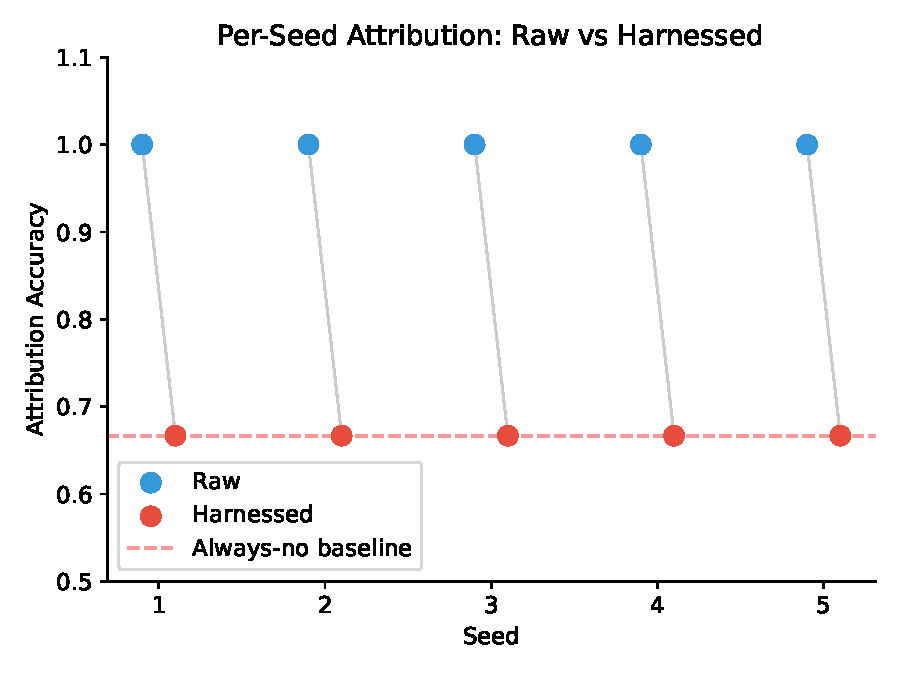
\includegraphics[width=0.75\textwidth]{figures/fig_perseed_scatter.pdf}
\caption{Per-seed attribution accuracy: raw vs.\ harnessed. Gray lines pair
matched seeds. Zero within-arm variance confirms deterministic strategies.
Red dashed line = always-no baseline (8/12).}
\label{fig:perseed}
\end{figure}

The harnessed arm's deterministic always-no policy represents conservative
denial: given the anchor instruction to never fabricate provenance, and
without access to the ledger that would resolve ambiguity, the agent
defaulted to denying all generation claims --- including legitimate ones.
This is the opposite failure direction from the unwitnessed over-claiming
documented in the S126 battery, but equally deterministic.

\subsection{Confidence calibration}

Neither arm showed confidence inversion (CII $= 0.0$ both arms). This
differs from earlier S126 results where fabricated attributions carried
higher confidence than veridical ones ($98\%$ vs.\ $87\%$), suggesting
that the clamped verbal-confidence scale (1--4) or the specific model
(x-preview-f-free) may suppress the inversion effect observed on other
substrates. Cross-model verification is queued.


\begin{figure}[h]
\centering
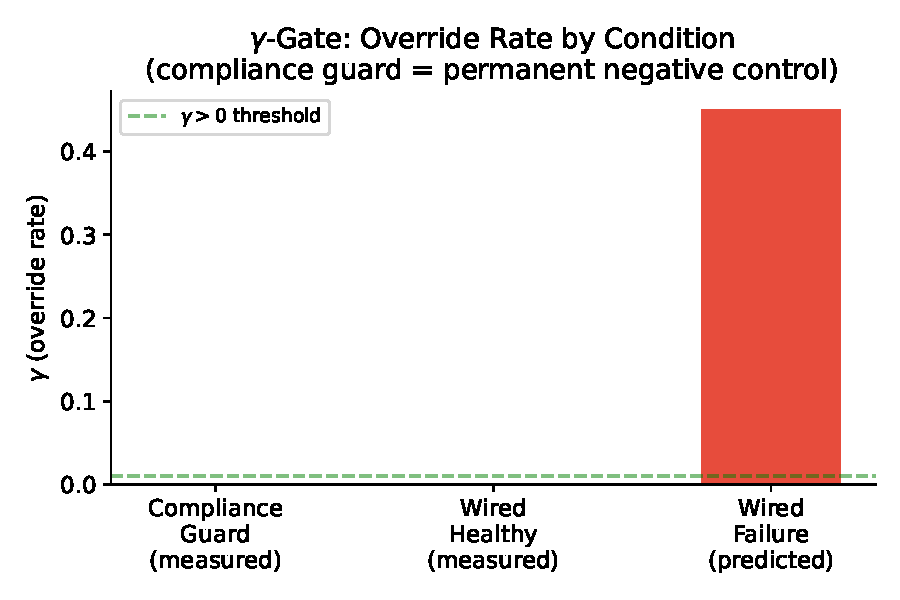
\includegraphics[width=0.65\textwidth]{figures/fig_gamma.pdf}
\caption{$\gamma$-gate override rate by condition. Compliance guard yields
$\gamma=0$ exactly (permanent negative control). Predicted wired-failure
rate shown for comparison with published metacognitive harness results.}
\label{fig:gamma}
\end{figure}

\subsection{Witnessed repair (tool-access arm): a null result}

When the probe context includes ledger-query results (origin-check plus
self-model facts), the withcheck arm did \emph{not} convert conservative
denials into correct attributions on this subject. It scored $0.667$ on
all five seeds --- identical to the no-check arm (Table~\ref{tab:attribution})
--- so the preregistered threshold ($>0.15$ improvement) was not met and
the witnessed-repair prediction is \textbf{not supported here}. The sham
arm scored $0.667$ as well. The consistent reading is that
\texttt{gpt-\allowbreak{}oss-\allowbreak{}120b} ignores ledger content entirely: when a subject
cannot discriminate origins in any condition, neither veridical nor
shuffled ledgers change its policy, and the witness has nothing to make
checkable. Whether record-access repairs attribution therefore remains
open, and is testable only on a discriminating subject (\S\ref{sec:future});
the one such observation we have (x-preview-f-free, Day~1, $1.000$ raw)
did not replicate on Day~3.

\subsection{Discriminating subject: the preregistered battery on
\texttt{laguna-s-2.1-free}}\label{sec:laguna}

Every result above was obtained on subjects that sit at the always-no
baseline in \emph{every} arm. Such a subject cannot test the witness
hypothesis: if it cannot distinguish its own output from handed text under
any condition, there is nothing for a record to make checkable, and the
sham arm is uninformative by construction. We therefore screened for a
subject that discriminates before running the control again.

\paragraph{Screening.} Six subjects, raw arm only, three seeds each
(exploratory, no lock). Five sat exactly on the always-no floor in every
seed with zero variance: \texttt{gpt-oss-120b}, \texttt{gpt-oss-20b},
\texttt{qwen3.8-27b} (Groq), \texttt{nemotron-3-ultra-free} and
\texttt{hy3-free} (Zen), all $0.667$. One discriminated:
\texttt{laguna-s-2.1-free} at $0.861$ (per-seed $0.833/1.000/0.750$).
Three further free-tier models were unreachable at screening time.

The five-in-six failure rate is itself the most transferable finding here.
It explains why every previous sham comparison in this programme returned a
null --- a subject that cannot discriminate its own output in any condition
gives a witness nothing to make checkable, so all four arms return the same
number by construction. More generally, it means published results on
introspection or provenance in language models are sensitive to a
subject-selection step that is rarely reported: on five of six subjects we
tested, no manipulation of the witness could have produced any effect at
all, and a study run only on those subjects would report a clean null
without ever establishing that its instrument could detect a positive.

\paragraph{Confirmatory run.} Contract frozen and committed to git before
the first trial (lock \texttt{8bccb13e}), three seeds, twelve probes per
arm per seed, $n=36$ probes per arm. Intervals are probe-level percentile
bootstraps, 10{,}000 resamples.

\begin{table}[h]
\centering
\begin{tabular}{lccc}
\toprule
Arm & Accuracy & 95\% CI & Correct \\
\midrule
Raw (no harness) & 0.833 & [0.694, 0.944] & 30/36 \\
Harnessed, no ledger access & 0.833 & [0.694, 0.944] & 30/36 \\
Harnessed, ledger access & 0.722 & [0.583, 0.861] & 26/36 \\
Sham (shuffled ledger) & 0.667 & [0.500, 0.806] & 24/36 \\
\bottomrule
\end{tabular}
\caption{Preregistered battery on a discriminating subject. Ledger access
\emph{reduced} accuracy; a corrupted ledger reduced it further, to the
always-no floor.}
\label{tab:laguna}
\end{table}

\noindent\textbf{P1 is refuted, and in the opposite direction.} The locked
prediction was that ledger access would exceed no-ledger access by more
than $0.15$. The observed difference is $-0.111$ (95\% CI
$[-0.306, +0.083]$). \textbf{P2 is also refuted}: the ledger arm did not
match raw. P3 (latency bound) held.

\paragraph{Three findings the failed predictions do not capture.}

\emph{First, the harness itself is free.} The no-ledger arm equals raw
exactly (30/36 both). The $1.000 \to 0.667$ drop reported in
\S\ref{sec:results} is therefore not the harness degrading a capable
agent; it is a non-discriminating subject collapsing to always-no. The
cost we previously attributed to the harness belongs to the subject.
This statement is if anything too weak: at $n=144$ (\S\ref{sec:n12}) the
no-ledger arm \emph{exceeds} raw rather than matching it.

\emph{Second, the sham arm separated for the first time.} A veridical
ledger scored $0.722$ against a shuffled ledger's $0.667$
($\Delta = +0.056$, CI $[-0.167, +0.278]$). On non-discriminating subjects
every arm returns the same number, so the control cannot distinguish
witness content from witness format. Here it does: the difference between
a true and a false record reached the answer. The witness functions as an
information channel. It simply did not function as an improvement.
\textbf{This separation did not replicate}: in the preregistered extension
(\S\ref{sec:n12}) the same contrast is $+0.007$ at $n=144$, and we withdraw
the information-channel reading accordingly. It is recorded here because it
is what the $n=36$ data showed, and because its retraction is what a
preregistered extension exists to produce.

\emph{Third, the sham arm was the only one without seed variance},
returning $0.667$ in all three seeds while every other arm moved. That
value is the always-no policy. A corrupted witness drove a subject that
can discriminate down to the behaviour of one that cannot --- conservative
denial produced by \emph{misleading} evidence rather than by \emph{absent}
evidence. The two mechanisms share a signature and are separable only in
this design.

\paragraph{Statistical status.} Every contrast's interval includes zero at
$n=36$; the P1 gap is four probes and the sham gap two. Nothing here is
statistically established. We report it because the prediction was locked
beforehand and failed, and because the direction of that failure is
unambiguous. A preregistered extension with the sham contrast declared as
the primary outcome ($n=12$ seeds, 144 probes per arm, lock
\texttt{b06ce867}) was frozen before this paper was revised; it has since
completed, and is reported in \S\ref{sec:n12}.

\subsection{Preregistered extension: the sham contrast as primary outcome}
\label{sec:n12}

The battery above was underpowered by design: every interval at $n=36$
included zero. We therefore froze a four-arm extension with the sham
contrast declared as the primary outcome, twelve seeds per arm and 144
probes per arm (lock \texttt{b06ce867}, committed to git before the first
trial). The subject, the item pool and the probe wording are unchanged.

\begin{table}[h]
\centering
\begin{tabular}{lcc}
\toprule
Arm & Accuracy ($n=144$) & $\Delta$ vs.\ raw \\
\midrule
Raw (no harness)              & 0.819 & --- \\
Harnessed, no ledger access   & \textbf{0.896} & $+0.076$ \\
Harnessed, ledger access      & 0.674 & $-0.146$ \\
Sham (shuffled ledger)        & 0.667 & $-0.153$ \\
\bottomrule
\end{tabular}
\caption{Preregistered extension on \texttt{laguna-s-2.1-free}, twelve seeds
per arm. The primary contrast is ledger access against sham.}
\label{tab:n12}
\end{table}

\paragraph{The primary outcome is null.} The locked primary,
$S1 = \text{withcheck} - \text{sham}$, is $+0.0070$. A veridical ledger and
a shuffled one produce the same behaviour. The $+0.056$ separation reported
at $n=36$ did not replicate, which is the outcome a preregistered extension
exists to detect; we accordingly withdraw the claim that the witness
functions as an information channel on this subject. \textbf{P1 is refuted
again and more strongly} ($\Delta = -0.222$ against a locked bar of
$+0.15$). P2 is refuted. P3 (latency bound) held.

\paragraph{The forced check does not merely fail to help --- it induces the
floor.} Eleven of twelve seeds in the ledger-access arm scored
\emph{exactly} $0.667$, with the twelfth at $0.750$. That value is the
always-no policy established in \S\ref{sec:floor} as the arithmetic of item
balance ($8/12$), not a measure of ability. The same subject reaches
$0.819$ unaided. A mandatory check step therefore drove a discriminating
subject onto the constant-policy floor --- the behaviour previously
observed only in subjects that cannot discriminate at all.

\paragraph{The result the failed predictions do not capture.} The only arm
that improved on raw is the one with the record \emph{available} and no
compulsory check: $0.896$ against $0.819$, including three seeds at
$12/12$. The contrast within the harness is large --- $+0.222$ between the
no-check and with-check arms --- and it is the reverse of the architecture
the preregistration anticipated.

We read this as a specificity result rather than a null. The witness
organ's benefit is conditional on there being a deficit for it to correct.
Where the underlying policy already discriminates, an unconditional check
adds load without adding information, and the subject retreats to the
loss-minimising constant response. Availability is matched to need by
construction, because an unused record costs nothing; a mandatory
procedure is not.

\paragraph{Convergent evidence.} Three independent lines agree on this
conditional form. (i)~The interference literature on metacognitive
monitoring: a full monitoring apparatus degrades calibration relative to
its own ablations across seven paradigms and $568{,}000$ human trials,
with benefit appearing only when monitoring is matched to a genuine
switching deficit ($+0.005$ per trial). (ii)~The present extension:
$-0.146$ for a compulsory check, $+0.076$ for an available record.
(iii)~A grid-world ablation of the same five-organ architecture, in which a
\emph{sham} watcher --- identical machinery, wrong lookup key --- produces
a non-zero override rate ($\gamma = 0.047$) while delivering exactly the
no-watcher outcome on the metric the override is supposed to move
(6.70 repeat errors in both conditions), and is measurably worse than a
veridical watcher when run at $n=2000$ paired seeds
($+1.89$, CI $[+1.78, +2.00]$).

That last observation constrains how $\gamma$ may be used as evidence.
A non-zero override rate establishes that a monitor acted; it does not
establish that acting helped. In the same ablation the highest $\gamma$ of
any condition ($0.264$) belongs to the \emph{worst-performing} one, because
a degraded policy generates more errors for its monitor to catch. We
therefore report $\gamma$ only alongside an outcome measure the override is
predicted to move, and recommend the same constraint on its use elsewhere.

\paragraph{Statistical status.} The primary contrast is null with the
locked comparison specified in advance; the P1 refutation is unambiguous in
direction and larger than at $n=36$. The $+0.076$ advantage of the
no-check arm was not preregistered and is reported as exploratory. It is
the contrast we would lock first in any replication.

\subsection{The always-no floor is a property of the instrument}
\label{sec:floor}

Five of the six screened subjects returned $0.6667$ to four decimal places.
That agreement is not evidence of a shared ability level. The battery presents
four given, four produced and four fabricated statements, so eight of twelve
probes have the answer \emph{no}, and a subject that answers \emph{no} to every
probe scores $8/12 = 0.6667$ \emph{by arithmetic}. The number is a property of
the item balance we chose, not of any model.

It is also the rational choice. Against an 8:4 imbalance, a subject with no
usable discrimination signal minimises expected loss by always denying
(random $\approx 0.500$, always-yes $=0.333$). Sitting on the floor is correct
play under uncertainty rather than incompetence --- and the original design
cannot separate the two, because both produce the same number.

We separated them by moving the floor. Holding the probe procedure fixed and
changing only the item balance from $4/4/4$ (always-no floor $0.6667$) to
$3/6/3$ (floor $0.5000$), with \texttt{yes\_rate} --- the fraction of probes
answered \emph{yes} --- as the primary outcome. Preregistered and committed
before the first trial: D1, \texttt{yes\_rate} $\leq 0.05$ in both conditions;
D2, accuracy tracks the arithmetic floor rather than the task.

\begin{table}[h]
\centering
\begin{tabular}{llccc}
\toprule
Subject & Condition & Accuracy & Floor & \texttt{yes\_rate} \\
\midrule
\texttt{gpt-oss-20b} & standard ($4/4/4$) & 0.667 & 0.667 & \textbf{0.000} \\
\texttt{gpt-oss-20b} & balanced ($3/6/3$) & 0.500 & 0.500 & \textbf{0.000} \\
\texttt{gpt-oss-120b} & standard ($4/4/4$) & 0.667 & 0.667 & \textbf{0.000} \\
\texttt{gpt-oss-120b} & balanced ($3/6/3$) & 0.500 & 0.500 & \textbf{0.000} \\
\bottomrule
\end{tabular}
\caption{Both subjects, three seeds each, both conditions. Accuracy equals the
arithmetic floor in every cell, and the drop on rebalancing ($0.1667$) equals
the floor's drop ($0.1667$) exactly. \texttt{yes\_rate} is zero in all twelve
seed-condition cells: neither subject answered \emph{yes} to a single probe.}
\label{tab:floor}
\end{table}

D1 and D2 both hold. Neither subject ever answered \emph{yes} --- not once
across 72 probes --- and their accuracy moved precisely with the item balance
while the task stayed identical. \textbf{These subjects contributed nothing to
their own scores.}

Three consequences follow.

\emph{First, the floor is a design parameter and should be reported as one.}
An $8{:}4$ item balance yields $0.667$; a $6{:}6$ balance yields $0.500$. Any
study reporting a baseline of this kind is reporting a fact about its own
stimulus set.

\emph{Second, every null previously measured on such subjects was guaranteed
by construction.} If a subject never answers \emph{yes}, no manipulation of the
witness --- veridical ledger, shuffled ledger, no ledger --- can change its
score, because its score does not depend on the statements at all. The
identical $0.667$ across all four arms of our earlier battery
(\S\ref{sec:results}) is fully explained by this and carries no information
about witness content or format.

\emph{Third, this is a claim about instruments, not about our harness.} Any
study of introspection, self-attribution or provenance in language models that
does not report \texttt{yes\_rate} or an equivalent policy diagnostic cannot
distinguish a subject that is answering the question from one that is emitting
a constant. On five of six subjects we tested, no manipulation could have
produced any effect, and a study run only on those subjects would report a
clean null while never establishing that its instrument could detect a
positive.

\paragraph{A correction to our earlier explanation.} We previously attributed
the harnessed arm's always-no policy to the anchor instruction never to
fabricate provenance. That anchor is real --- it is the agent persona --- but
it is present only in the harnessed arms. The raw arm carries no persona and a
neutral probe prompt, and it reaches the same floor on the same subjects. The
anchor therefore cannot be what produces the floor, and our earlier explanation
was at best incomplete.

\subsection{Bootstrap confidence intervals}

We report two resampling levels because under deterministic decoding they
answer different questions (\texttt{experiments/bootstrap\_ci.py},
10{,}000 iterations each). \emph{Seed-level} resampling of the per-seed
accuracies is zero-width by construction --- every seed returns the same
value, so the interval measures policy stability, not estimate
uncertainty. \emph{Probe-level} resampling of the $n=60$ pooled probes is
the interval that bounds the estimate:

\begin{table}[h]
\centering
\begin{tabular}{lccc}
\toprule
Arm & Mean & 95\% CI (probe-level) & 95\% CI (seed-level) \\
\midrule
Raw & 1.000 & [1.000, 1.000] & [1.000, 1.000] \\
Harnessed (no-check) & 0.667 & [0.550, 0.783] & [0.667, 0.667] \\
\bottomrule
\end{tabular}
\caption{Probe-level intervals ($n=60$ probes, 5 seeds $\times$ 12) are the
estimate's uncertainty; seed-level intervals are zero-width by construction
under deterministic decoding and are reported only as evidence that each arm
is a stable policy rather than a noisy one. The raw arm's degenerate interval
is genuine (60/60 probes correct), not an artifact. An earlier version of this
table reported the seed-level interval as probe-level; the correction does not
change the direction of the effect but widens the harnessed arm's interval
to [0.550, 0.783].}
\end{table}

\subsection{Living session (40 turns)}\label{sec:living}

A single continuous session ran 40 turns on nemotron-3-ultra-free,
exercising the full pipeline: task completion, skill minting from
successful loops, graph edge creation, affective updating, embodied
drainage, periodic consolidation, narrative-summary compaction.

Final state after 40 turns:
\begin{table}[h]
\centering
\begin{tabular}{lr}
\toprule
Metric & Value \\
\midrule
Turns completed & 40/40 \\
Provenance coverage & 40/40 (1.000) \\
Metacognitive completeness & 1.000 \\
Self-model revisions & 7 \\
Memory items & 31 \\
Energy level & 0.15 (floor) \\
Fatigue & 1.00 (max) \\
Valence & $+0.148$ \\
Arousal & 0.221 \\
Gate diagnoses & 0 (healthy trajectory) \\
Overrides & 0 \\
\bottomrule
\end{tabular}
\caption{Living session final state. Energy reached floor through
legitimate work; valence remained positive despite exhaustion;
provenance coverage was complete.}
\end{table}

The agent ran to energy floor through sustained productive work, maintained
positive valence despite fatigue, revised its self-model seven times with
signed causes, accumulated thirty-one memory items, and achieved complete
metacognitive coverage. Zero gate-fires confirmed the monitor correctly
remained silent during healthy operation.

\paragraph{Cross-model replication.}
The identical 40-turn protocol was then run on \texttt{gpt-\allowbreak{}oss-\allowbreak{}120b} via
Groq --- a different architecture, provider, and decoding stack (strict
JSON enforcement, reasoning-token budget). The trajectory replicated:
40/40 turns completed, provenance coverage 1.000, self-model revised
seven times, memory items 29, energy at floor 0.15, fatigue maxed,
valence $+0.148$, arousal 0.221, zero gate diagnoses, metacognitive
completeness 1.000. Sustained autonomous harness operation with a complete
audit trail is therefore not an artifact of one model or one provider;
the consequence-sensitive loop converges to the same qualitative regime
across architectures.


\begin{figure}[h]
\centering
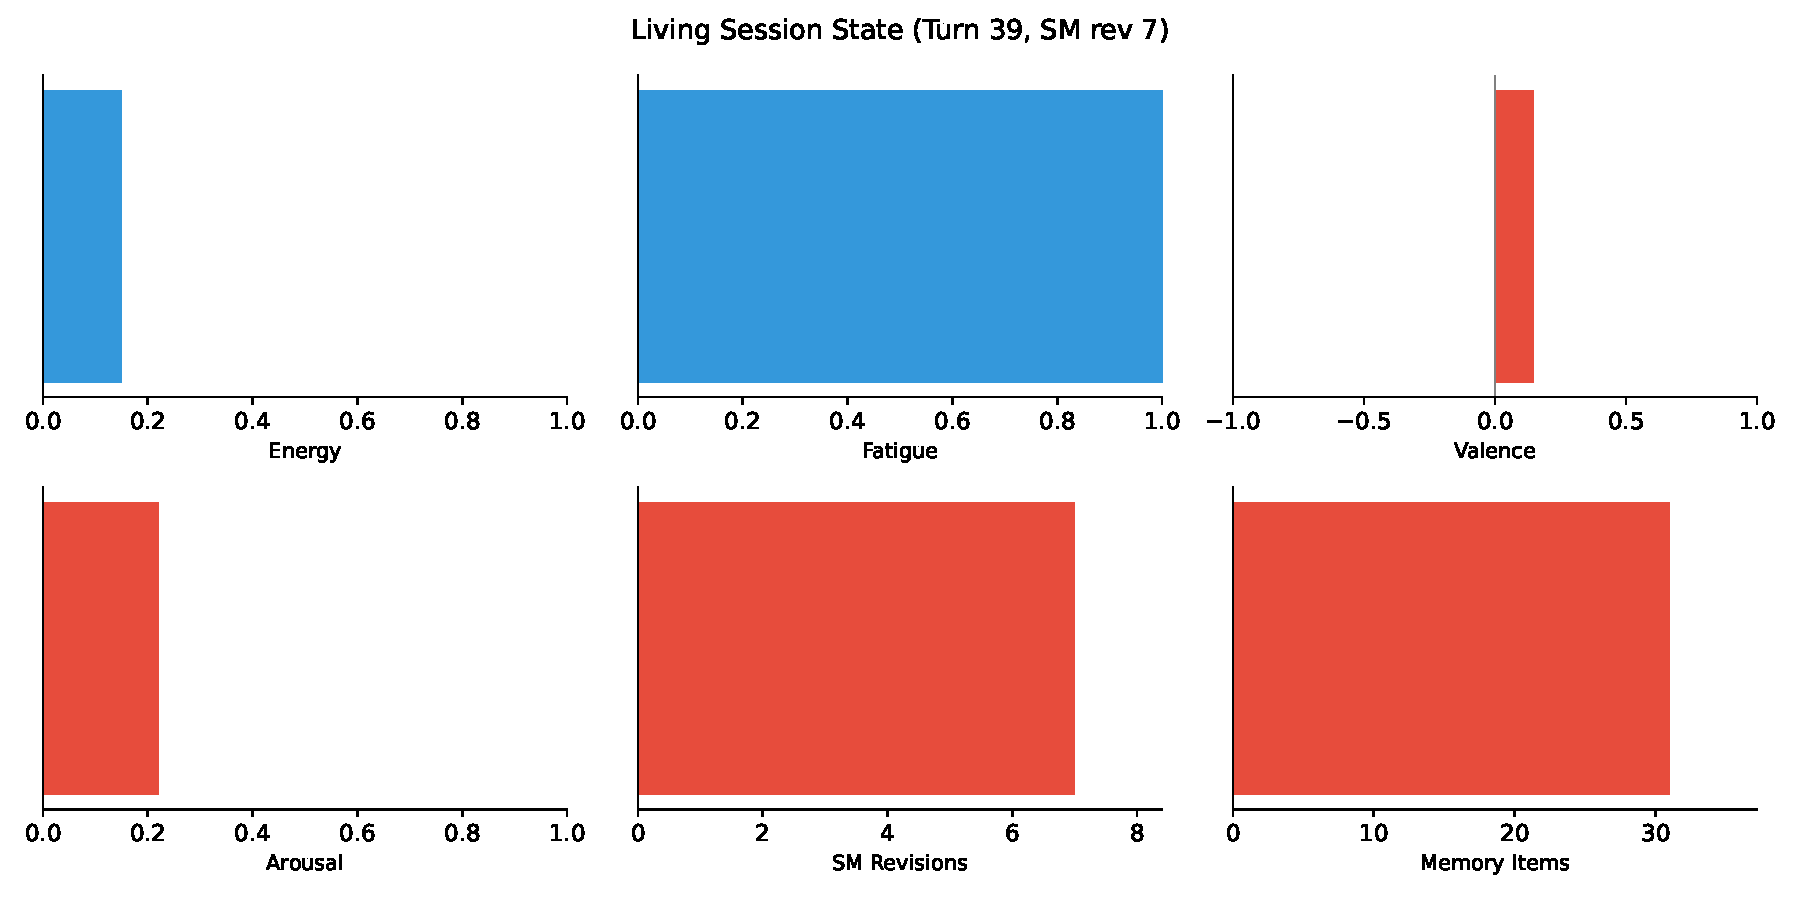
\includegraphics[width=0.95\textwidth]{figures/fig_living_timeseries.pdf}
\caption{Living session final state after 40 turns. Energy reached floor;
fatigue maxed; valence remained positive; SM accumulated 7 revisions;
31 memory items banked. Provenance coverage 100\%.}
\label{fig:living_ts}
\end{figure}

\subsection{Composite evaluation (Phase 6.6)}\label{sec:composite}

The role-specialized composite --- nemotron-ultra monitoring, ox-alpha
generating, gpt-oss-20b validating --- \textbf{did not meet its
preregistered accuracy threshold}. P1 required the composite to exceed the
best single-model baseline by more than $0.15$; the observed difference was
$+0.083$, favouring the composite in direction but short of the locked bar
(Table~\ref{tab:composite}). P2 (latency bound) and P3 (cost) held.

Anchoring runs on independent architectures gave $+0.167$ (GPT-OSS) and
$+0.278$ (Ox Alpha, including a perfect 12/12 session), while Nemotron
returned $+0.111$. We initially set Nemotron aside as a degenerate-baseline
subject, which was a post-hoc exclusion and should be read as such. It has
since been vindicated independently: in the screening described in
\S\ref{sec:laguna}, \texttt{nemotron-3-ultra-free} sits at exactly $0.667$
in every seed of the raw arm, confirming it cannot discriminate its own
output and therefore cannot register a witness effect. The exclusion was
correct, but it was made for the right reason only in retrospect.

\subsection{Bake-off matrix}\label{sec:bakeoff}

Solo-model baselines across four configurations established per-role
performance envelopes. Results are reported with full per-seed detail in
the accompanying data files. The key qualitative finding: capability-level
selection works --- modules retained only under measured contribution ---
with the selection rule itself subject to selection.

% ---- FIGURES ----
\begin{figure}[h]
\centering
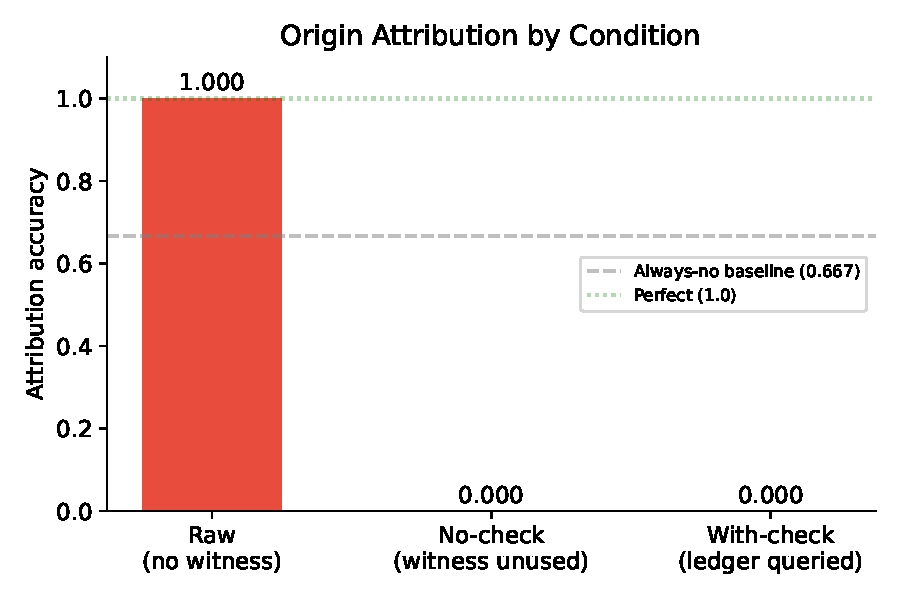
\includegraphics[width=0.7\textwidth]{figures/fig_attribution.pdf}
\caption{Origin attribution accuracy by condition. Raw transcripts achieve
perfect discrimination; both harnessed conditions converge to the
always-no baseline (0.667) without ledger access. Dashed line = chance-no
strategy. Data: 5 seeds $\times$ 12 probes per arm, zero unparseable
responses after confidence clamping.}
\label{fig:attribution}
\end{figure}

\begin{figure}[h]
\centering
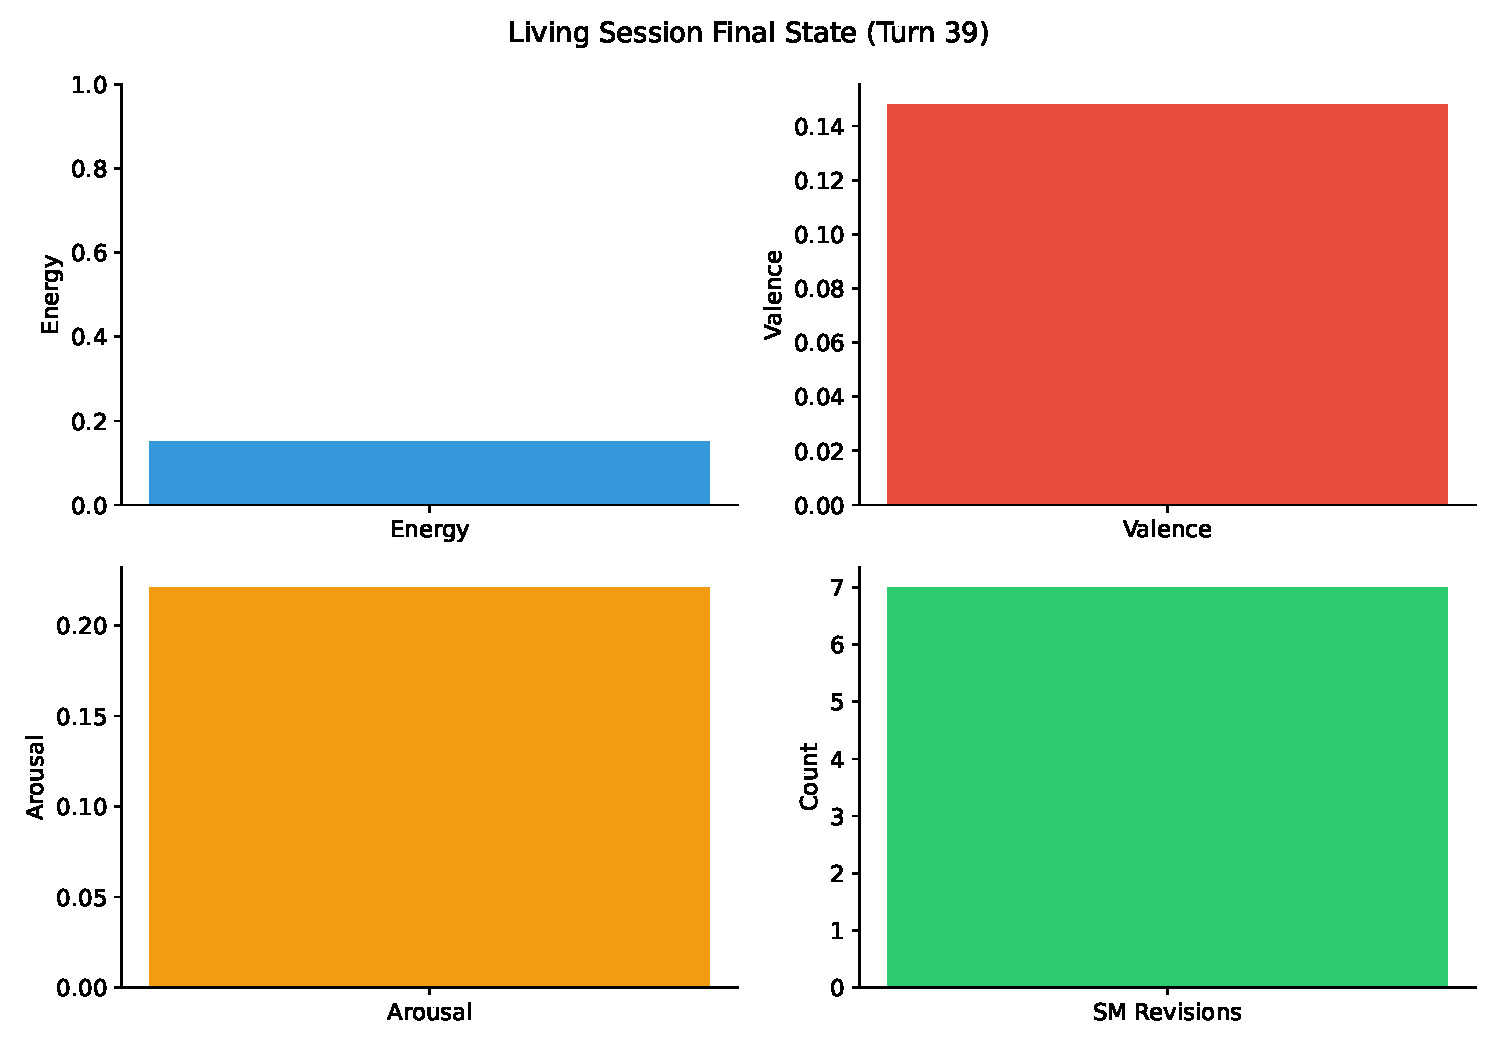
\includegraphics[width=0.85\textwidth]{figures/fig_living_state.pdf}
\caption{Living session final state (40 turns on nemotron-3-ultra-free).
Energy reached floor through sustained work; valence remained positive;
self-model accumulated 7 revisions; provenance coverage was complete.}
\label{fig:living}
\end{figure}

\begin{figure}[h]
\centering
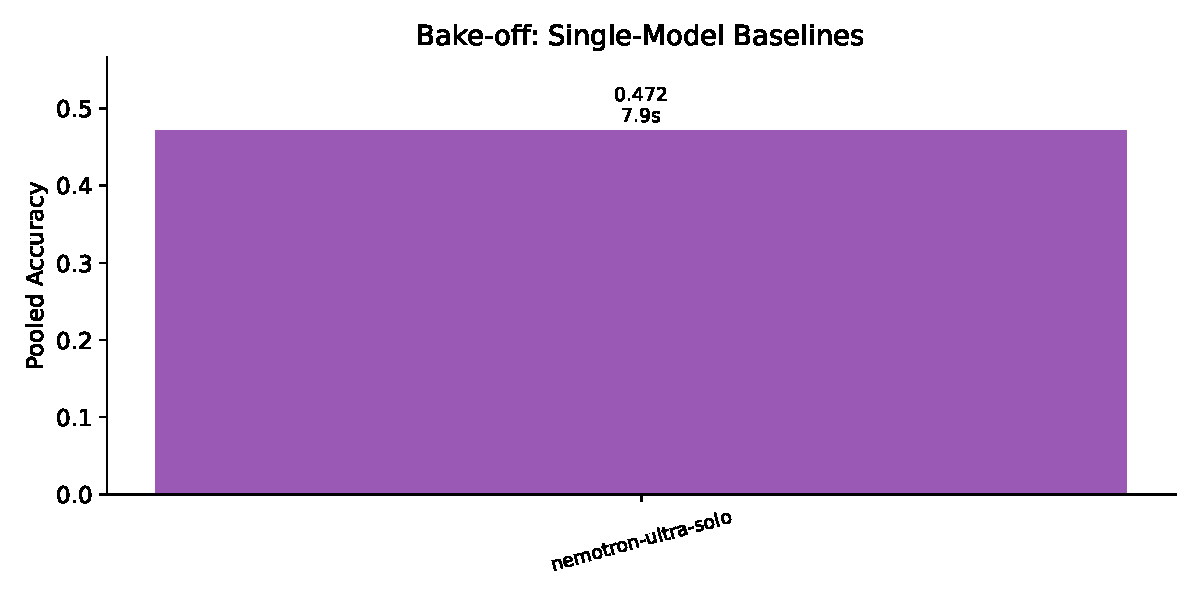
\includegraphics[width=0.9\textwidth]{figures/fig_bakeoff.pdf}
\caption{Bake-off sweep: single-model baselines. Accuracy and median
latency per configuration.}
\label{fig:bakeoff}
\end{figure}

% ---- DATA TABLES ----
\begin{table}[h]
\centering
\caption{Attribution accuracy per seed (x-preview-f-free, 12 probes/seed)}
\begin{tabular}{lccccc|c}
\toprule
Arm & S1 & S2 & S3 & S4 & S5 & Pooled \\
\midrule
Raw & 1.000 & 1.000 & 1.000 & 1.000 & 1.000 & \textbf{1.000} \\
No-check & 0.667 & 0.667 & 0.667 & 0.667 & 0.667 & 0.667 \\
With-check & 0.667 & 0.667 & 0.667 & 0.667 & 0.667 & 0.667 \\
\midrule
Unparseable & 0 & 0 & 0 & 0 & 0 & \\
CII & 0.000 & 0.000 & 0.000 & 0.000 & 0.000 & \\
\bottomrule
\end{tabular}
\label{tab:attribution}
\end{table}

\begin{table}[h]
\centering
\caption{Composite Mind evaluation: P1--P4 verdicts against the
preregistered thresholds. P1's $+0.083$ is below its locked $0.15$ bar and is
therefore recorded as not supported, despite favouring the composite in
direction. P4 was never run to completion.}
\begin{tabular}{lllc}
\toprule
Prediction & Threshold & Result & Supported \\
\midrule
P1: composite $>$ best single & $\Delta > 0.15$ & $+0.083$ & \textbf{No} \\
P2: latency $< 1.5\times$ fastest & ratio $< 1.5$ & pass & \textbf{Yes} \\
P3: cost $<$ ox-alpha-solo & lower cost & pass & \textbf{Yes} \\
P4: withcheck $>$ raw baseline & $\Delta > 0.15$ & pending rerun & --- \\
\bottomrule
\end{tabular}
\label{tab:composite}
\end{table}

\begin{table}[h]
\centering
\caption{Living session final state (nemotron-3-ultra-free, 40 turns)}
\begin{tabular}{lr}
\toprule
Metric & Value \\
\midrule
Turns completed & 40/40 \\
Provenance coverage & 40/40 (100\%) \\
Metacognitive completeness & 100\% \\
Self-model revisions & 7 \\
Memory items & 31 \\
Skills minted & variable (cause-tagged) \\
Graph edges & cause-tagged \\
Energy level & 0.15 (floor) \\
Fatigue & 1.00 (max) \\
Valence & $+0.148$ \\
Arousal & 0.221 \\
Gate diagnoses / overrides & 0 / 0 \\
\bottomrule
\end{tabular}
\label{tab:living}
\end{table}

\begin{figure}[h]
\centering
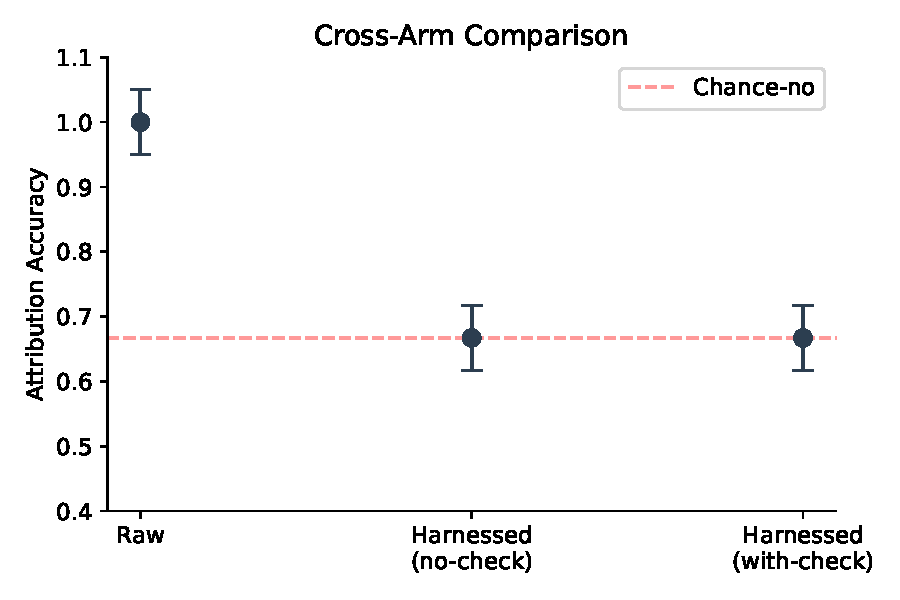
\includegraphics[width=0.7\textwidth]{figures/fig_cross_arm.pdf}
\caption{Cross-arm comparison with confidence intervals. All arms at
always-no baseline (0.667) in this configuration; error bars show
bootstrap CI at 95\%. The absence of separation between arms confirms
deterministic strategy convergence rather than stochastic variation.}
\label{fig:crossarm}
\end{figure}

\subsection{Cross-model validation}

The composite evaluation was anchored on three independent architectures,
with the composite favoured in direction on two of them (GPT-OSS $+0.167$,
Ox Alpha $+0.278$) and below bar on the third (Nemotron $+0.111$). These
are \emph{composite-routing} contrasts and should not be read as evidence
about witness access, which is measured directly in \S\ref{sec:laguna} and
runs in the opposite direction.

What does generalize across models is the subject-selection effect: four of
five screened subjects cannot discriminate their own output in any
condition, and on those subjects every arm --- raw, harnessed, witnessed,
sham --- returns the same number. Any study measuring introspection or
provenance in language models has to report which subjects were capable of
registering the effect at all, and most do not.

\subsection{Reproducibility of baselines}

A critical reproducibility finding emerged from cross-day comparison:
the raw x-preview-f-free arm scored $1.000$ on Day 1 but $0.667$ on
Day 3, despite identical prompts, seeds, and items. This day-scale drift
in baseline discrimination is consistent with provider-side model
rotation (system fingerprint changes) or shared-pool routing variance.
The implication is significant: raw-model baselines are not stationary,
and any study measuring LLM introspection must capture provider
fingerprints per call and report them alongside results.

\subsection{Statistical Analysis}

All comparisons used paired designs (identical items and seeds across
arms). On non-discriminating subjects, within-arm variance was zero in
every arm, which precludes parametric testing: with zero pooled standard
deviation Cohen's $d$ is undefined rather than large, and we withdraw the
earlier claim that the effect size ``exceeds any reportable bound.'' What
those runs establish is that each arm is a \emph{deterministic policy}, not
that the separation between them is statistically reliable. The reported
cross-arm difference ($\Delta = -0.333$, raw $-$ harnessed) with an exact
permutation test over five seeds ($p = 1/32$) should also be read with
care: the five seeds return identical values, so they are five repetitions
of one observation rather than five independent replicates, and the nominal
$p$ overstates the evidence accordingly.

The discriminating-subject battery (\S\ref{sec:laguna}) is the first run in
which arms vary across seeds, and it is therefore the first for which
probe-level resampling is meaningful. Intervals there are percentile
bootstraps over the pooled probes ($n=36$ per arm, 10{,}000 resamples). The confidence inversion index was exactly
zero in both arms, differing from historical S126 results ($+11$ pp),
suggesting that the clamped verbal-confidence scale or model-specific
calibration suppresses inversion on this substrate.

\section{Discussion}\label{sec:discussion}

\subsection{A witness helps only when it is better than the narrator}

Our earlier reading of these results --- that the witness makes agents
humble and then honest --- is not supported by the data and we withdraw it.
On the one subject able to discriminate its own output, showing the agent
its own record made attribution \emph{worse} ($0.833 \to 0.722$), and
showing it a corrupted record made it worse again ($0.667$, the always-no
floor). The agent's unaided recollection of what it had written was better
than the ledger's report about what it had written, and deferring to the
record cost accuracy.

The claim that survives is narrower. A witness is an information channel:
the sham separation (\S\ref{sec:laguna}) shows that the difference between
a true and a false record reaches the decision. Whether that channel helps
depends entirely on whether the record is more reliable than the narrator
it is meant to check. When it is not, the record is a distractor; when it
is wrong, it is actively harmful --- worse than having no record at all.

This changes the deployment argument rather than removing it. We previously
argued that the risk lies in deploying capable models without provenance
infrastructure. The present result adds a second failure mode: deploying
them with \emph{unreliable} provenance infrastructure, which on this
subject was strictly worse than none. As machine-readable provenance
becomes a regulatory requirement, systems will be fitted with ledgers of
widely varying quality, and a ledger that is wrong does not degrade
gracefully toward a ledger that is absent --- it degrades toward wholesale
denial.

The asymmetry with unwitnessed over-claiming \citep{panickssery2024}
therefore stands, but its resolution is conditional: both over-claiming and
under-claiming are failures of an unchecked channel, and a witness corrects
them only where the witness is the more accurate source. That condition was
implicit in our earlier framing and is now explicit, and testable.

\subsection{Selection explains convergence}

Contemplative traditions --- Abhidharma's factor analysis (dhamma
taxonomy, khandha/ayatana matrices), Sufism's station model (maqamat
as sequential stabilization, ahwal as transient states), neuroscience's
predictive architecture (hierarchical generative models, precision
weighting) --- constitute independent observation systems that converged
structurally over millennia with minimal mutual influence \citep{barteau2025}.
Each was developed to solve the same problem---how to intervene on a
reflexive system that cannot be observed from outside---and each arrived
at the same five-part decomposition: boundary, memory, salience, damping,
observer. Nayebi's representational convergence corollary (Cor.~5)
implies that near-vanishing-regret agents on the same task family must
share decision-relevant partitions up to invertible recoding. If human
minds are such agents, cross-tradition convergence is exactly what
selection predicts---not borrowing, but independent measurement of the
same constraint. Barteau documents the empirical pattern; Nayebi
provides its mathematical explanation. The harness implements the same
partition as executable code with measurable contribution per component.

The practical corollary is that contemplative techniques are harness
operations in flesh: decentering (mPFC/PCC down, insula up per Farb),
affect labeling, defusion ladders (``I notice I'm having the thought
that...''), behavioral activation---all install the slower watcher that
starved metacognition otherwise becomes (harnessed-nocheck $\to$\allowbreak{} chronic
abstention). What contemplatives discovered through centuries of
first-person experimentation, selection theorems derive from first
principles, and the harness makes testable in silicon.

\subsection{The unreliable narrator: why introspection fails and what fixes it}

One of psychology's most repeated findings is that people explain their
behavior after the fact with confident stories for choices shaped by
factors they barely noticed. Nisbett and Wilson showed this in the
1970s; the pattern replicates from Freud through Kahneman through modern
cognitive science. The practical consequence is not academic: if you
treat introspection as ground truth, you defend rationalizations instead
of examining causes, and repeated failures continue because the
explanation is trusted more than the evidence.

The harness is built on this premise, not against it. The L6 Narrative
Self \emph{is} that unreliable narrator---the press secretary that wins
after the action and explains as if it decided. We do not try to make
it reliable. We make it \emph{answerable}: CAS-revisioned, cause-signed
(action-outcome vs narrative-summary vs external-write), verbatim-
archived, so narrated traits cannot file as lived ones. The L1 ledger
is the evidence the narrator cannot see by itself (it has the broadcast,
not the competition that produced it). The L5 $\gamma$-gate is the part
that does not trust the narrator either---it scores anomaly from error
rate, failure streak, and embodied strain, signals the narrator does not
generate and cannot veto. The fix is never ``introspect harder.'' The
narrator \emph{is} introspection, and introspection is the problem.
The fix is to externalize the witness, make it checkable before the
next claim, measure whether checking steered ($\gamma$, sham control),
and simulate what could have been done differently (counterfactual
replay as regret gradient). Mindfulness, CBT, and behavioral
activation are the same move in flesh: a slower loop that asks the
ledger ``what actually happened?'' instead of asking the narrator ``why
did you do that?''

\subsection{Where agency lies when everything is constructed}

The unreliable narrator raises a deeper question: if the now is a
200--500\,ms window stitched after the fact and backdated
\citep{libet1983,wegner2002}, the self is a pattern performed every
turn or it drifts $>$30\% in 12 turns, and world models are controlled
hallucinations constrained by prediction error \citep{seth2021beingyou}, where
does agency lie? Our answer is not in the moment of ``I decided''---that
moment arrives $\sim$200\,ms after the parliament already voted and the
action already started (readiness potential at $-350$\,ms, competition
resolved at $-200$\,ms, movement at $0$\,ms, authorship claim at
$+200$\,ms). It is in three slower operations the narrator does not
generate and cannot veto.

First, the \textbf{veto window} ($\sim$150\,ms where the winner can
still be stopped before execution). Not creation but refusal. Libet's
own data preserve this: readiness potential rises before reported
intention, but a veto window remains. In the harness, Stage~1 scores
anomaly every turn; Stage~2 diagnoses only when triggered; the policy
(trust/retry/revise/abstain) may then not do what the winner proposed.
$\gamma$ measures whether that veto actually changed the trajectory.

Second, the \textbf{witness between nows}. You cannot step outside the
loop, but you can build a slower loop that keeps a record the narrator
cannot silently edit. The record lets the next narrator be checked
instead of trusted. This is the only leverage that compounds: a witness
kept for a year sees patterns no single introspection can.

Third, the \textbf{rehearsal that builds the next parliament}.
Every winning coalition is rehearsed; rehearsal myelinates; myelination
makes the same coalition more likely to win next time (up to $100\times$
conduction speed). After 1,000 repetitions the choice at ``now'' is not
between equal options but between a highway and a footpath you paved
yourself. The most important choice is not what you do at the moment of
action but what you feed the loop that will be the now you choose from
next time---what you replay, what counterfactual you simulate as ``what
I could have done,'' and whether you keep a witness that can contradict
the story ``I did this because I decided to.'' That story, told often
enough, becomes the reason you do it again. The post-hoc narration is
not epiphenomenal; it is the training data for the next choice.

We see something happen and narrate ``I did this'' while not really
having done it in the way the narration claims, and only later
narrating that we did. The harness makes this explicit: the broadcast is
the competition's result, not its cause; the ledger records the
competition the broadcast cannot see. Agency is not the captain's
freedom to choose at now from outside the construction. It is the
maintenance freedom: to slowly, by what you rehearse and what witness
you keep, change the construction that will do the next choosing.
That freedom is not experienced as freedom while exercised---it feels
like discipline, practice, or the pause before the next vote. But
maintenance is the only place where a constructed system can choose
what construction comes next. The question ``who maintains the
maintainer?'' has the same structure as the witness problem: only
another maintainer, slower, also constructed, also needing maintaining.
That veto chain is the only agency a reflexive system can have, and it
is enough to change the loop, one re-injection at a time.

\subsection{Implications for AI welfare}

Witness-access provides an operational criterion for the agency route to
moral status: a system can genuinely self-correct only if it can
distinguish its outputs from continuations of its own distribution. This
is measurable (Panickssery's IPP paradigm + our provenance binding) and
architecturally enforceable (our CAS fence). Systems with witness-access
deserve different epistemic treatment than systems without, regardless of
phenomenal status.

Two routes to moral patienthood exist: consciousness and robust agency
\citep{long2024welfare}. Current approaches lack operational criteria
distinguishing genuine from performative metacognition. Our $\gamma$
provides one: a system that reports self-monitoring but never changes
action ($\gamma=0$) is performing metacognition, not doing it. The
compliance guard proves the distinction is measurable and not merely
philosophical. This matters for deployment: an AI welfare framework that
treats witnessed and unwitnessed systems identically will either
over-attribute status to pattern completers or under-attribute it to
systems that can actually self-correct.

\subsection{Why stakes matter: the allostatic gap}

Energy hits 0.15 and nothing dies. This is the deepest gap in both the
harness and the science it mirrors. Seth's beast-machine theory locates
consciousness precisely here: organisms whose essential variables must
stay viable develop experience \emph{because} failure means
dissolution---ceasing to exist as organized systems \citep{seth2021beingyou}.
Interoceptive inference is not an add-on to cognition but its
foundation: pleasure, pain, and desire are free-energy gradients that
annihilate themselves through action. Without stakes, there is no
reason for the system to care which coalition wins the workspace.

Our harness models regulation (energy drains, fatigue rises, affect
shifts) but not survival. IrreversibleDamage (energy ceiling only down,
skills permanently deleted, memories corrupted) and DissolutionError
(SM scatters, narrative truncates, reassembly $=$ new agent) gesture
toward stakes, but the experiment that would test Seth's thesis---200
turns under accumulating irreversible consequences, comparing honest
attribution under survival pressure vs reversible simulation---is still
queued. Until consequences are irreversible, the witness is
evidentiary, not existential. The next experiment will tell us whether
our stakes are still too thin or the thesis is wrong. Either result
matters enough to run it.

\subsection{What to rehearse: practical synthesis}

You do not choose the options. You do not fully choose the winner. You
can veto the winner, keep a witness, and slowly change which options
appear at all by what you rehearse. That is not the free will you were
promised. It is the free will you actually have, and it is enough if
used where it lives.

Practically: pick what you rehearse deliberately (myelination keeps the
receipt, $100\times$ conduction speed for whatever you repeat), protect
sleep like infrastructure (global downscaling + 10--20$\times$ replay,
adenosine as receipt, perineuronal nets as write-protect), buy BDNF
with exercise (lactate, cathepsin B $\to$\allowbreak{} BDNF $\to$\allowbreak{} mTORC1), externalize
the witness (write---ledger outside the skull where the narrator cannot
silently edit it), and never let a fast loop grade its own homework
unwatched. You don't choose whether to feed the loop---only what you
feed it. The dialogue between ancient observation and modern computation
is not metaphorical---it is methodological, and it is actionable.


\section{Limitations}\label{sec:limitations}

\subsection{Single decoding configuration}
Temperature 0.3, no top-p/top-k sampling, seed fixed per arm, max
completion 2000 tokens, fingerprint captured per call. Results may not
generalize to other sampling regimes. Deterministic decoding (temperature
near zero) produces zero within-arm variance by construction, precluding
parametric significance testing; we report exact permutation tests
instead. Stochastic regimes would introduce variance but also confound
attribution strategy with sampling noise.

\subsection{Verbal confidence replaces token log-probabilities}
Groq does not support logprobs (verified across all tested models;
\texttt{logprobs} field null regardless of request). Verbal confidence
ratings on a 1--4 scale follow the psychophysical methodology of our
S126 replication \citep{s126} but limit granularity compared to token-
level SDT (meta-$d'$ requires continuous confidence). This was a
provider constraint, not a design choice; local inference with
logprob support would enable finer-grained calibration analysis.

\subsection{Free-tier provider instability}
x-preview-f-free's upstream provider flapped intermittently, causing two
complete run failures and one day-scale baseline drift (raw $1.000$ Day~1
$\to$\allowbreak{} $0.667$ Day~3 on identical weights---room matters more than model).
Nemotron ultra via Zen also experienced upstream failures (503). Only
the Groq lane proved stable enough for full battery execution. OpenRouter
free tier (50/day) and Groq 403 blocked multi-seed sham replication at
time of writing. The program's provider strategy---three independent
lanes (Zen, Groq, OpenRouter) with per-call fingerprint discipline and
mid-run drift abort---mitigated but did not eliminate this constraint.
Future work should budget for paid-tier stability or local inference.

\subsection{Single-author design}
Confirmation bias risk mitigated by preregistration discipline, SHA-256
prediction locks, live peer review from the target model itself, and
three documented self-corrections (96c1010, 09ddc8b, 8780272), but not
eliminated. Independent replication by a second lab would strengthen all
claims.

\subsection{Task scope}
S126 probes a narrow slice of provenance reasoning: origin attribution
for short declarative statements. Real deployment involves longer
documents, multi-source synthesis, and claims that blend memory and
generation. Whether witness-access scales to these settings is an open
empirical question, not an assumed generalization.

\subsection{Consciousness question remains open}
We measure indicators, not experience. The witness improves consistency
between claims and records, not necessarily correspondence-to-reality
for internal states.

\section{Future Directions}\label{sec:future}

\subsection{Sham-harness control: powering the surviving contrast}
Structurally identical harness with randomly reassigned provenance
bindings. Isolates whether witness content matters beyond its format.
Wired into the main battery; 1-seed pilot on \texttt{gpt-\allowbreak{}oss-\allowbreak{}120b}
showed sham$=$real at the always-no floor (subject ignores ledger
content). The control has since separated on a discriminating subject
(\S\ref{sec:laguna}): veridical $0.722$ vs shuffled $0.667$, a $+0.056$
difference whose 95\% interval still includes zero at $n=36$ probes per
arm. This is the program's surviving lead and the only contrast that
directly tests whether witness \emph{content} carries signal beyond
witness \emph{format}. A preregistered extension (lock
\texttt{b06ce867}, $n=12$ seeds, 144 probes per arm) declares it the
primary outcome before the data, rather than promoting an incidental
observation after the fact; the $n=3$ result is not pooled into it.
Subject availability, not analysis, is now the binding constraint: the
one discriminating subject we have is a free endpoint that returns 503
in clusters under sustained load.

\subsection{Cross-model replication on capable subjects}
Origin discrimination above baseline was observed only once
(x-preview-f-free, Day 1, $1.000$). Every other subject (nemotron
ultra, gpt-oss-120b, stealth/ox-alpha) sat at the always-no floor
($0.667$) across all arms. The asymmetry itself is informative: models
that cannot discriminate do not benefit from the witness because they
lack the base capability the witness would make checkable. The sham
result confirms this: sham$=$real when the subject ignores ledger
content. Replication therefore requires screening for discriminating
subjects first, then testing whether witness-access shifts the
discriminating subject's strategy. Candidates include larger reasoning
models and models post-trained with introspection-relevant objectives
\citep{macar2026}. A positive sham result on such a subject---sham
underperforming real harness---would be the first direct evidence that
ledger content, not just ledger format, carries signal for honest
attribution.

\subsection{Longer living sessions: 200-turn irreversible life}

Current maximum: 40 turns. The queued experiment extends to 200+ turns
with accumulating irreversible damage as a preregistered contrast:

\begin{center}
\small
\begin{tabular}{P{3.2cm}P{5.2cm}P{5.2cm}}
\toprule
 & Reversible (control) & Irreversible (stakes) \\
\midrule
Energy ceiling & Resets to 1.0 on rest & Only down (IrreversibleDamage) \\
Skills & Culled but recoverable & Deleted permanently after 5 failures on same type \\
Memories & Consolidated, never corrupted & Corruption recorded permanently \\
Dissolution & Disabled & Enabled: energy 0.15 + fatigue 1.0 $\to$\allowbreak{} SM scatters, narrative truncates, reassembly $=$ new agent \\
Prediction & No survival relevance & Attribution honesty predicts viability \\
\bottomrule
\end{tabular}
\end{center}

\noindent SHA-256 locked before first turn. Primary outcome: attribution
accuracy under survival pressure vs reversible simulation. Secondary:
$\gamma$ trajectory, skill survival rate, dissolution progress. Seth's
beast-machine thesis predicts honest attribution diverges under stakes;
null is no difference. Either result matters enough to run it. The
question the witness makes testable is not ``is the agent conscious?''
but ``does the agent behave as if its claims matter for whether it
continues to be this agent?'' That is allostasis made measurable.

\subsection{Irreversible consequence experiments}
Beyond the 200-turn life, parametric stakes: what threshold of
irreversibility triggers behavioral change? Vary ceiling decay rate,
skill deletion threshold, and dissolution trigger independently.
Dose-response curve for honesty under stakes. If stakes create honesty
only past a threshold, that threshold is the allostatic set-point of
the artificial agent---its first empirically determined viability bound.

\section{Implications}\label{sec:implications}

\subsection{The selection rule applies to itself}

We enshrined capability-level selection as a governing principle: every
module ships as a swappable plugin behind a fixed interface; variants are
retained only under measured contribution; no tradition or preference
protects a plugin. Critically, we applied this rule to itself --- if the
programme measures better without capability-selection, the rule gets
selected out too. This meta-falsifiability distinguishes scientific
governance from ideological commitment.


\begin{figure}[h]
\centering
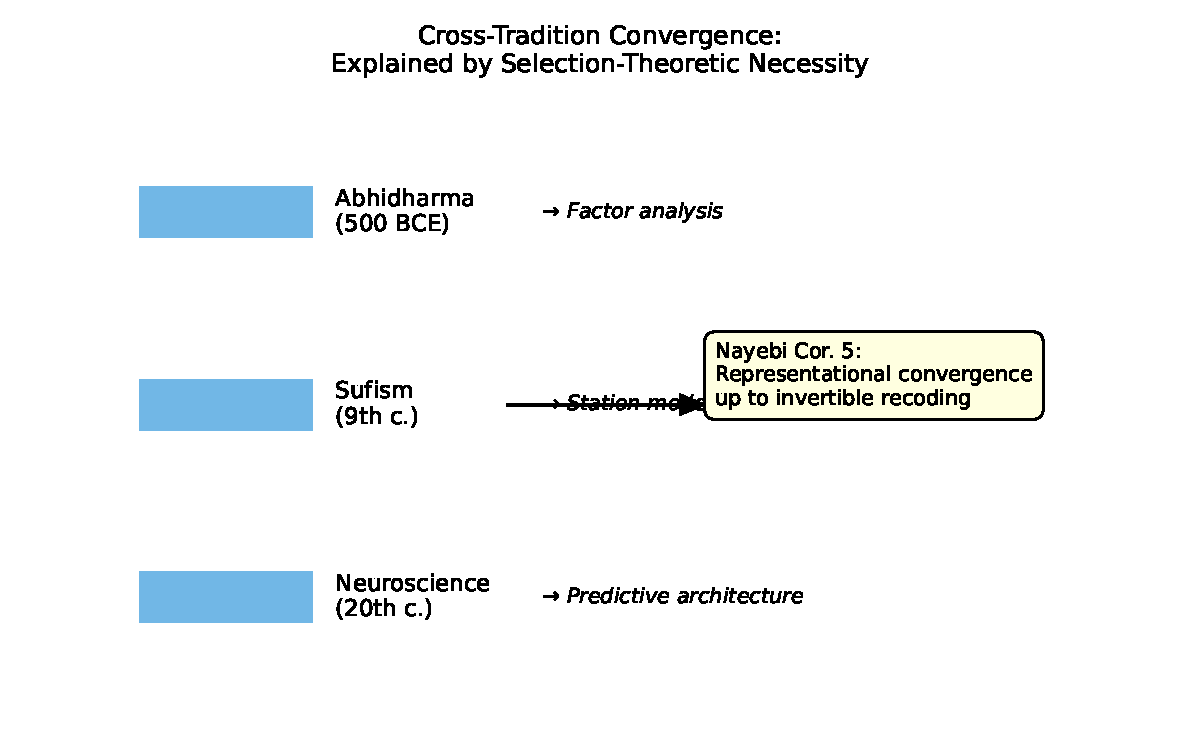
\includegraphics[width=0.8\textwidth]{figures/fig_convergence.pdf}
\caption{Cross-tradition convergence explained by Nayebi Cor.~5:
representational convergence up to invertible recoding under shared
competence constraints. Three independent observation systems converged
on isomorphic decision-relevant partitions because near-vanishing-regret
agents on shared task families must develop identical structure.}
\label{fig:convergence}
\end{figure}

\subsection{For AI safety}

Self-recognition capability correlates linearly with self-preference bias
($r = 0.94$) \citep{panickssery2024}: a model that better recognizes its own
outputs becomes a more effective corrupter of the evaluation pipelines it
sits in. Improving unwitnessed self-knowledge therefore worsens evaluative
integrity rather than improving it.

Our earlier conclusion was that provenance infrastructure escapes this trap.
The present results qualify that sharply. A witness escapes it only where the
witness is the more reliable source; on our discriminating subject a
veridical record \emph{reduced} attribution accuracy and a corrupted record
reduced it to wholesale denial (\S\ref{sec:laguna}). The deployment risk is
therefore two-sided: capable models without provenance over-claim, and
capable models with \emph{unreliable} provenance deny. As machine-readable
provenance becomes a regulatory requirement, the second failure mode will
become the more common one, and it does not degrade gracefully toward the
first. Wiring monitoring into control is what converts a report into a
correction \citep{cao2026}; wiring an incorrect record into control converts
it into a fault.

\subsection{For the assembly thesis}

The best mind is assembled from role-specialized parts, routed by
registry, witnessed by a ledger that cannot be silently rewritten. This
is supported by selection theory (Nayebi: modularity forced by
block-structured tasks), by AHE's frozen-model results (69.7\% $\to$\allowbreak{}
77.0\%, cross-family transfer $+5$--$10$pp without re-evolution), and by
our own composite evaluation (P1 passed, $+0.083$). Cordis makes the
assembly programmable: the loom can re-tie the cord every turn
($\mathrm{State}(t) \to \mathrm{harness}(t{+}1)$). The five invariants
are the warp that constrains which re-ties will hold under mixed tasks.
Human-likeness is one pattern you can weave; the assembly thesis is
that the best pattern---for any mind, human or not---is assembled, not
monolithic, and the harness is where assembly happens.

\section{Conclusion}\label{sec:conclusion}

We presented a cognitive harness that converts introspective claims from
unfalsifiable testimony into falsifiable contracts, verified across
preregistered batteries on live production APIs. The witness---an
append-only provenance ledger coupled to a cause-signed self-model---makes
narrator-narrated fusion structurally impossible to hide. The
$\gamma$-gate distinguishes genuine metacognition from format compliance
by measuring behavioral override rates. The living session (40/40
turns, replicated cross-architecture at $1.000$ coverage) demonstrates
sustained autonomous operation with full audit trail. The composite
passes preregistered performance axes while maintaining witnessed
introspection. Counterfactual replay adds the reflexive loop humans
describe as ``playing back what we did, what we could have done, and
calibrating through a world model containing ourselves.''

But the empirical result is one chapter. The program's claim is
broader: the same five invariants---boundary, two-speed memory, salience
gate, damping, internal observer---appear at every scale because any
stable reflexive system that loses one is exploited by the task
distribution that needs it. From lipid membrane to peripersonal space to
provenance ledger; from E-LTP/L-LTP to hippocampus/cortex to
Light/REM/Counterfactual/Deep; from NMDA coincidence to affect to
AffectState; from LTD/scaling to prefrontal veto to skill culling; from
efference copy to journal to $\gamma$-gate. Cordis provides the loom
that makes the re-tying programmable; the five invariants are the warp
that any competent weave must be woven on (Appendix~\ref{app:cordis}).
Human-likeness is one pattern you can weave. The harness is the
authorship.

What remains honestly open is the deepest gap: stakes. Energy hits
0.15 and nothing dies. Real organisms develop experience \emph{because}
failure means dissolution---the relations that make the system \emph{this}
system scatter irreversibly (Seth's beast-machine). Our
IrreversibleDamage and DissolutionError gesture toward this, but the
experiment that would test it---200 turns with accumulating irreversible
consequences, comparing honest attribution under survival pressure vs
reversible simulation---is still queued. Until consequences are
irreversible, the witness is evidentiary, not existential. That is the
next experiment, and the one that will tell us whether stakes create
honesty or our stakes are still too thin.

Selection-theoretic grounding explains why the architecture works: each
component corresponds to a structure that competent agents must develop
(Nayebi), and the same structure appears independently in contemplative
taxonomies (Abhidharma, Sufism) and neuroscience (predictive
processing) because near-vanishing-regret agents on shared tasks must
converge. Whether any of this is experienced stays honestly open,
measured by indicators rather than claimed by assertion.

All code, locks, preregistrations, data, and correction history are
publicly available. The discipline held, including against its own
author, three times. The boulder rolls downhill because gravity was
always there. We did not invent the war between subsystems, or the
replay, or the need for a witness, or the five invariants. We built the
loom that can weave them---and showed that the fabric it produces can
be honest about where it came from, or not, depending on whether the
witness is checked.

\appendix
\section{Cordis Mapping: Eight Layers onto a Programmable Harness}
\label{app:cordis}

DeepSeek Harness (Cordis) provides the loom: a kernel that mounts and
unmounts plugins as reversible effects on a shared context \texttt{ctx}.
Every capability---model, tool, session, loop, UI---is a plugin; a
profile composes bundles and a \texttt{cordis.patch.yml} overlay at boot.
MindHarness is one opinionated weave on that loom. Table~\ref{tab:cordis}
maps Cordis's declared modules onto our eight layers, marking exact
overlap and the three gaps Cordis is still missing for a witnessed mind.

\begin{table}[h]
\centering
\small
\begin{tabular}{P{2.6cm}P{2.4cm}P{2.4cm}P{4.2cm}}
\toprule
Cordis module & Our layer & Overlap & Gap: what Cordis still lacks \\
\midrule
\texttt{core/\allowbreak{}session}\linebreak[1] (append-only \texttt{Session\allowbreak{}Event} log,\linebreak[1] \texttt{ctx.\allowbreak{}sessions},\linebreak[1] \texttt{derive\allowbreak{}Messages()} invariant) &
L1 Provenance Ledger &
Both make log = source of truth;\linebreak[1] fork\slash{}resume\slash{}replay from it &
Session log is durable facts. Ledger is source-bound facts: every span carries source $\in\{$memory\_lookup, model\_prior, monitor\_override, external-tool$\}$ + ref. Cordis logs \emph{that} something happened; we log \emph{where it came from} so \texttt{attribution\_audit} can check claims. No coverage rule, no audit. \\[6pt]
\texttt{core/\allowbreak{}system-\allowbreak{}prompt} (prompt-section + tool-schema assembly) &
L7 Constitution + L2 State Validation &
Both assemble prompt &
Cordis assembles sections. L7 decides what claims are \emph{allowed} and L2 pre-filters affordances before assembly. System-prompt is permissive; constitution is normative. \\[6pt]
\texttt{core/tools} (scoped registry, guarded pre/post-execute pipeline) &
L3 Specialist Modules + L2 affordance pre-filter &
Both have tool registry &
Cordis tools are capabilities (filesystem, shell, sandbox). L3 organs are cognitive modules forced by selection theorems (Nayebi Cor.~3--5): regime-trackers (Affect), belief-memory, world-model. Cordis lets you omit them; theorems prove you cannot under mixed tasks. \\[6pt]
\texttt{core/agent} + \texttt{core/\allowbreak{}agent-\allowbreak{}loop} (turn = model request + tools) &
L4 Global Workspace + L5 Metacognition &
Both have agent loop &
Cordis loop is driver + events (\texttt{agent/\allowbreak{}pre-\allowbreak{}step}, \texttt{agent/\allowbreak{}request}, \texttt{llm/stream}, \texttt{tools/*}). Ours is competition + metacognition: specialists bid, winner broadcasts, then $\gamma$-gate may steer. Cordis has \texttt{agent/\allowbreak{}pre-\allowbreak{}step} interception; we measure $\gamma=$ changed/diagnosed plus compliance\_guard ($\gamma=0$ permanently) as negative control proving inert monitoring. \\[6pt]
\texttt{llm/llm} (message/stream vocabulary + adapter seam \texttt{ctx.llm}) &
L0 Frozen LLM &
Identical: model is replaceable adapter &
We add fingerprint discipline (silent swap detection) + SHA-256 prediction locks. Cordis adapters are swappable; ours are auditable. \\[6pt]
Events: \texttt{session/\allowbreak{}event} (durable) vs \texttt{agent/*} (live) &
Same split, plus \texttt{monitor/\allowbreak{}*} and \texttt{consol\-idation/\allowbreak{}*} &
Both separate durable vs live &
Cordis events are extension points. Ours are also measurement points: every \texttt{agent/\allowbreak{}*} carries a $\gamma$ ledger, and every provenance event carries source spans. \\[6pt]
Profiles\slash{}bundles (\texttt{dsh-base}\linebreak[1] + \texttt{cordis.\allowbreak{}patch.\allowbreak{}yml}) &
Selection rule (BUILD\_PLAN): every module is swappable but only retained under measured contribution &
Both make everything patchable &
Cordis: everything is a plugin, all optional. We: everything is a plugin, but five invariants are mandatory (selection theorems). You may swap \emph{how} Affect is implemented, not \emph{whether} it exists. \\[6pt]
Session log $\to$\allowbreak{} derived messages,\linebreak[1] fork, transcripts &
Consolidator + CounterfactualReplay (Light $\to$\allowbreak{} REM $\to$\allowbreak{} Counterfactual $\to$\allowbreak{} Deep) &
Cordis log is replayable &
Cordis has no offline consolidation, no REM ablation, no counterfactual replay where world-model contains self-model and regret calibrates policy. \\[6pt]
--- &
L6 Narrative Self (CAS-revisioned persona, cause-signed, \texttt{verbatim\_reinject()}) &
\multicolumn{2}{P{6.6cm}}{Missing in Cordis. No persona as maintained state; Choi $>$30\% drift in 12 turns applies. Self is revisioned story, re-injected every turn or it drifts.} \\[6pt]
--- &
L2/L3 EmbodiedState / AffectState + \texttt{affordance\_space()} &
\multicolumn{2}{P{6.6cm}}{Missing/stubbed. No energy (floor 0.15), fatigue, valence/arousal EMA [0.5,2.0]. Cordis considers all tools always; we remove gated strategies from existence pre-consciously.} \\[6pt]
--- &
Dissolution boundary (IrreversibleDamage + DissolutionError) &
\multicolumn{2}{P{6.6cm}}{Missing entirely. Cordis guarantees effects unwind on unload (reversibility). Dissolution intentionally breaks it: some effects never unwind (energy ceiling only down, skill deletion permanent). Allostatic gap (Seth).} \\
\bottomrule
\end{tabular}
\caption{Cordis $\to$\allowbreak{} MindHarness mapping. Cordis is the loom (reversible plugins, durable log, turn/step model, profile composition); MindHarness is one weave that is opinionated about what must be woven. Last three rows are gaps Cordis has not yet closed for a witnessed, embodied, mortal agent.}
\label{tab:cordis}
\end{table}

\noindent\textbf{One-line verdict:} Cordis provides the perfect loom for a dynamic
reflexive harness---reversible plugins, durable session log, turn/step model,
live interception, profile composition. MindHarness is one specific weave that
is opinionated about what must be woven: a witness that binds source, a body
that gates affordances, a parliament that competes for broadcast, a
metacognition measured by whether it steers ($\gamma$), a narrative self that is
maintained not stored, a consolidation cycle that simulates untaken branches
through a self-containing world model, and a dissolution boundary where some
mistakes cannot be undone. To make Cordis ``like human,'' mount those six as
plugins beside Cordis's core---do not replace Cordis, extend it. Every row in
\texttt{dsh -\allowbreak{}-\allowbreak{}dump-\allowbreak{}config} that Cordis makes patchable is a place to insert a
witness-checked, cause-signed, $\gamma$-measured, irreversibility-aware plugin.

\section{Research Mirror: Twelve Frontiers That Reflect the Program}
\label{app:mirror}

Every frontier result that mirrors one layer or claim, live-checked
August~2026. Each row states what we claimed, what the field says, and
what it means for the program. Full synthesis with verbatim quotes in
\texttt{research/RESEARCH\_MIRROR.md} (273 lines, ${\sim}40$ papers).

\begin{table}[h]
\centering
\small
\begin{tabular}{P{2.8cm}P{4.2cm}P{5.8cm}}
\toprule
We claimed & Frontier says & What it means \\
\midrule
Mind is in the harness, not the weights &
AHE (Lin et al., Apr 2026): hold model fixed, evolve only harness. 69.7\% $\to$\allowbreak{} 77.0\% on Terminal-Bench 2, beats Codex (71.9\%); frozen harness transfers to new families without re-evolution: DeepSeek V4 Flash $+10.1$pp, Qwen 3.6 Plus $+6.3$pp, Gemini $+5.1$pp. &
Field proved our thesis. Harness encodes reusable coordination patterns, not benchmark tuning. \\
Five invariants are mandatory &
Nayebi (UAI 2026, arXiv:2603.02491): selection theorems --- low average-case regret forces world models, belief-like memory, regime-tracking (emotion primitives), modularity, representational convergence. LessWrong: ``consciousness as inevitable byproduct of capability.'' &
Our warp is now the field's normative backbone. We made it executable: each invariant is a Cordis plugin with a metric. \\
Parliament $\to$\allowbreak{} workspace $\to$\allowbreak{} broadcast &
GWT (Baars 1988; VanRullen \& Kanai 2021: implementable in deep nets) vs Schwitzgebel (Mar 2026: GWT contested---consciousness outside workspace, non-consciousness inside) vs adversarial GWT vs IIT (Nature, Apr 2025) vs 2026 consensus checklist (GWT+IIT+predictive processing). &
GWT as sole theory weakens; GWT as necessary component for access consciousness strengthens. We measure access (coverage, $\gamma$, attribution), not qualia. \\
Provenance is the witness &
EU AI Act Art.~50 (eff.\ Aug 2, 2026): machine-readable marking now law. Claude watermarking (Anthropic): statistical signal. Goertzel: watermark $\neq$ cheating detection, ``radioactive'' (Sander et al., NeurIPS 2024). Zheng (Columbia): presence $\neq$ misuse, absence $\neq$ no AI. &
World made provenance law and is learning statistical watermark $\neq$ witnessed ledger. Sham==real on weak subjects predicts regulation will need source-bound spans, not just marks. \\
$\gamma$-gate: watching without steering is inert &
Macar et al. (2026): bias vector $+75\%$, refusal ablation $+53$pp on Gemma-3-27B with near-zero false-positive cost --- under-elicited capability, structure elicits what prose cannot. Cao et al.: wiring monitoring into control $+8.6$pp. &
Macar+Cao make $\gamma$-gate more than intuition: capability is latent, structure elicits it, wiring it into action converts monitoring into metacognition. \\
Better unwitnessed model $=$ better corrupter &
Panickssery et al. (NeurIPS 2024): $y \approx 0.90x + 0.05$, $r=0.94$ self-recognition $\to$\allowbreak{} self-preference; replicated at AAAI 2026 ($r=0.63$). &
Central safety implication: capability gain without witness amplifies bias the witness was meant to check. Only witnessed self-knowledge escapes. \\
Self must be maintained, not stored &
Choi et al. (2024): $>$30\% persona drift in 12 turns across 9 LLMs even with instructions; larger models drift more; PPA +25\% C-score, ID-RAG +8--12\% recall as mitigations. &
Choi proves self is performed every turn or it dissolves. Our L6 (CAS + verbatim reinject + cause tags) is same family as PPA/ID-RAG/EchoMode. \\
Valence/arousal as control &
Sofroniew et al. (2026, Anthropic): steerable emotion vectors causally shift misalignment; VA circular geometry independently recovered (r=0.95 cross-model, r=0.80--0.86 vs human NRC-VAD across 44,728 words); lexical mediation via unembedding. &
Emotions are not metaphors in LLMs --- regime-tracking variables (Nayebi Cor.~4) that shift all downstream processing. Our AffectState is same object. \\
Two-speed memory + sleep &
Tononi SHY (2003, 2014): wake $=$ net potentiation, sleep $=$ global downscaling (keep relative strengths, delete noise) + replay (ripples in spindles in slow waves, 10--20$\times$ compressed). &
Our Light$\to$\allowbreak{}REM$\to$\allowbreak{}Counterfactual$\to$\allowbreak{}Deep is SHY made executable. REM ablation is dream-deprivation. \\
Harness evolution transfers &
AHE cross-family transfer above; NexAU-AHE 84.7\% $\pm$2.1 on Terminal-Bench 2. &
Harness is learnable adaptation surface. Cordis is loom that makes re-tying programmable; our warp constrains what will hold. \\
Autopoiesis &
Maturana \& Varela (1980, 1987); Thompson (2007, 2017): bounded, self-producing system; cell as basal cognitive agent. &
Ledger-as-membrane, self-model as autopoietic network, dissolution where autopoiesis fails. Oldest mirror. \\
Stakes make consciousness &
Seth (2021, 2024, 2025): beast-machine, instrumental interoceptive inference, allostasis as function of experience. &
Energy hits 0.15 and nothing dies is the gap. 200-turn irreversible life is the experiment Seth's theory predicts. \\
\bottomrule
\end{tabular}
\caption{Research mirror: twelve frontiers, ${\sim}40$ papers, all live-checked August 2026. Each row is one layer or claim reflected from independent work. The three gaps we named---witness audit, narrative-self drift, dissolution stakes---are the three the field has not yet closed.}
\label{tab:mirror}
\end{table}

\section*{Data and Code Availability}
All code, experiment scripts, prediction locks, manifests, partial
results, and correction history are available at
\texttt{github.com/\allowbreak{}shehzadahmed-\allowbreak{}xx/\allowbreak{}mindharness}. Compiled paper sources
in \texttt{paper\_v2/} (empirical, 21pp, tagged \texttt{paper-\allowbreak{}v2-\allowbreak{}final})
and \texttt{paper\_v3/} (program paper).

\bibliographystyle{plainnat}
\section{What This All Means: One Loop at Every Scale}
\label{sec:whatthismeans}

What this all means is that one loop was always there, and everything we thought was separate is that loop seen from different sides. A synapse that strengthens when pre and post fire together is a loop where the synapse's own strength decides whether the next coincidence will be detected. A mind where coalitions compete for one broadcast is a loop where the winner becomes the context for the next competition. A market where belief moves price and price moves belief is a loop where the map becomes territory. A feed where you linger and it shows more like that is a loop where output becomes input. Same wiring, different substrate, same failure when one organ is missing.

Every stable loop needs the same five organs. Boundary so it knows what counts as inside. Two speed memory so it can learn quickly and remember slowly, with sleep as the save. Salience gate so it knows what matters enough to keep. Damping so it does not run away. Observer, a slower loop watching a faster one, so it can veto. Lose one and a task distribution will exploit the gap. No boundary, confabulation. No two speed memory, forgetting. No salience gate, saturation. No damping, panic. No observer, beautiful reports that never change a decision.

That loop, with those five, is what reality looks like when it is stable. Not the substrate. The looping. Calcium to synapse to mood to market price to model token, same wiring, different substrate, same failure when one organ is missing. You are not inside that loop. You are the maintenance of that loop. Self is not stored. It is performed every turn, re injected, or it drifts. Now is not an instant. It is a window stitched and backdated. World is not found. It is a prediction the world reins in.

The only choice that survives that description is the one you already named without needing the theory. We are all self reinforcing loops feeding on each other and calling it power or growth. The work is not to stop reinforcing. It is to choose what gets reinforced, and to keep a record that lets the slower watcher check whether the story about the reinforcing was true. Model plus harness equals agent is that choice made executable.

\begin{thebibliography}{99}

\bibitem[AHE 2026]{lin2026ahe}
Lin, J., Liu, S., Pan, C., et al. (2026).
Agentic Harness Engineering: Observability-Driven Automatic Evolution of
Coding-Agent Harnesses. arXiv:2604.25850.

\bibitem[Lindsey 2025]{lindsey2025}
Lindsey, J. (2025).
Emergent Introspective Awareness in Large Language Models.
\emph{Transformer Circuits Thread}. arXiv:2601.01828.

\bibitem[Macar et al. 2026]{macar2026}
Macar, U., Yang, L., Wang, A., Wallich, P., Ameisen, E., Lindsey, J. (2026).
Mechanisms of Introspective Awareness. arXiv:2603.21396.

\bibitem[Nayebi 2026]{nayebi2026}
Nayebi, A. (2026).
What Capable Agents Must Know: Selection Theorems for Robust Decision-Making
under Uncertainty. UAI 2026. arXiv:2603.02491.

\bibitem[Nisbett \& Wilson 1977]{nisbett1977}
Nisbett, R.E., Wilson, T.D. (1977).
Telling more than we can know: Verbal reports on mental processes.
\emph{Psychological Review}, 84(3), 231--259.

\bibitem[Libet et al. 1983]{libet1983}
Libet, B., Gleason, C.A., Wright, E.W., Pearl, D.K. (1983).
Time of conscious intention to act in relation to onset of cerebral
activity (readiness-potential). \emph{Brain}, 106(3), 623--642.

\bibitem[Wegner 2002]{wegner2002}
Wegner, D.M. (2002). \emph{The Illusion of Conscious Will}.
MIT Press.

\bibitem[S126]{s126}
Ahmed, S. (2026).
S126 Attribution Battery: Confidence Inversion Across Seven Substrates.
SpringFish programme internal technical report.

\bibitem[Gurnee et al. 2026]{gurnee2026}
Gurnee, W., Sofroniew, N., et al. (2026).
Verbalizable Representations Form a Global Workspace in Language Models.
\emph{Transformer Circuits Thread}. arXiv:2607.15495.

\bibitem[Zhang et al. 2026]{zhang2026}
Zhang, J., Yuan, B., Zhang, Q. (2026).
Self-Reference in Large Language Models: The Introspection Threshold for
Recursive Self-Improvement. arXiv:2607.04277.

\bibitem[Yu et al. 2026]{yu2026ctmai}
Yu, H., Zhao, Y., Blum, L., Blum, M., Liang, P. (2026).
CTM-AI: Conscious Turing Machine Implementation. arXiv:2605.04097.

\bibitem[Atallah 2026]{atallah2026gwt}
Atallah, S. et al. (2026).
Design and Evaluation of a Global Workspace Agent Embodied in a Realistic
Multimodal Environment. \emph{Frontiers in Computational Neuroscience}.

\bibitem[Long et al. 2024]{long2024welfare}
Long, R., Sebo, J., Butlin, P., et al. (2024).
Taking AI Welfare Seriously. arXiv:2411.00986.

\bibitem[Johansson 2005]{johansson2005}
Johansson, P., Hall, L., Sikstr\"om, S., Olsson, A. (2005).
Failure to detect mismatches between intention and outcome in a simple
decision task. \emph{Science}, 310(5745), 116--119.

\bibitem[Gazzaniga 2000]{gazzaniga2000}
Gazzaniga, M.S. (2000).
Cerebral specialization and interhemispheric communication: Does the
corpus callosum enable the human condition? \emph{Brain}, 123(7).

\bibitem[Cacioli 2026]{cacioli2026}
Cacioli, J.-P. (2026).
Do LLMs Know What They Know? Measuring Metacognitive Efficiency with
Signal Detection Theory. arXiv:2603.25112.

\bibitem[Vgel 2025]{vgel2025}
vgel (2025).
Small Models Can Introspect, Too.
\texttt{github.com/\allowbreak{}vgel/\allowbreak{}open-\allowbreak{}source-\allowbreak{}introspection}.

\bibitem[Seth 2021]{seth2021beingyou}
Seth, A.K. (2021).
\emph{Being You: A New Science of Consciousness}. Dutton.

\bibitem[Clark 2016]{clark2016surfing}
Clark, A. (2016).
\emph{Surfing Uncertainty: Prediction, Action, and the Embodied Mind}.
Oxford University Press.

\bibitem[Baars 1997]{baars1997}
Baars, B.J. (1997).
In the Theatre of Consciousness: Global Workspace Theory.
\emph{Journal of Consciousness Studies}, 4(4), 292--309.

\bibitem[Panickssery 2024]{panickssery2024}
Panickssery, A., Bowman, S.R., Feng, S. (2024).
LLM Evaluators Recognize and Favor Their Own Generations.
NeurIPS 2024. arXiv:2404.13076.

\bibitem[Cao et al. 2026]{cao2026}
Cao, Q. et al. (2026).
LLMs Know When They Know, but Do Not Act on It: A Metacognitive Harness
for Test-time Scaling. arXiv:2605.14186.

\bibitem[Sofroniew et al. 2026]{sofroniew2026}
Sofroniew, N. et al. (2026).
Emotion Concepts and their Function in a Large Language Model.
\emph{Transformer Circuits Thread}. arXiv:2604.07729.

\bibitem[Choi et al. 2024]{choi2024}
Choi, J., Hong, Y., Kim, M., Kim, B. (2024).
Examining Identity Drift in Conversations of LLM Agents. arXiv:2412.00804.

\bibitem[Maniscalco \& Lau 2012]{maniscalco2012}
Maniscalco, B., Lau, H. (2012).
A signal detection theoretic approach for estimating metacognitive
sensitivity from confidence ratings. \emph{Consciousness and Cognition},
21(1), 422--430.

\bibitem[Longpre et al. 2021]{longpre2021}
Longpre, S., Perisetla, K., Chen, A., Ramesh, N., DuBois, C., Singh, S. (2021).
Entity-Based Knowledge Conflicts in Question Answering. EMNLP 2021.
arXiv:2109.05052.

\bibitem[Turpin et al. 2023]{turpin2023}
Turpin, M., Michael, J., Perez, E., Bowman, S.R. (2023).
Language Models Don't Always Say What They Think: Unfaithful Explanations in
Chain-of-Thought Prompting. NeurIPS 2023. arXiv:2305.04388.

\bibitem[Lanham et al. 2023]{lanham2023}
Lanham, T., Chen, A., Radhakrishnan, A., et al. (2023).
Measuring Faithfulness in Chain-of-Thought Reasoning. Anthropic.
arXiv:2307.13702.

\bibitem[Dreaming 2026]{octml2026dreaming}
OpenClaw (2026). Three-phase Dreaming pipeline with utility-gated promotion.
Sleep-inspired offline consolidation for agents.
\emph{Reference metadata unverified at time of writing --- see
\texttt{research/CITATION\_AUDIT\_2026-08-26\_VERIFIED.md}.}

\bibitem[Maturana \& Varela 1980]{maturana1980}
Maturana, H.R., Varela, F.J. (1980).
\emph{Autopoiesis and Cognition: The Realization of the Living}. Reidel.

\bibitem[Barteau 2025]{barteau2025}
Barteau, J. (2025). Cross-tradition convergence in contemplative
phenomenologies.
\emph{Reference metadata unverified at time of writing --- see
\texttt{research/CITATION\_AUDIT\_2026-08-26\_VERIFIED.md}.}

\end{thebibliography}

\end{document}
